\begin{figure}[H] \centering % !TEX encoding = UTF-8 Unicode
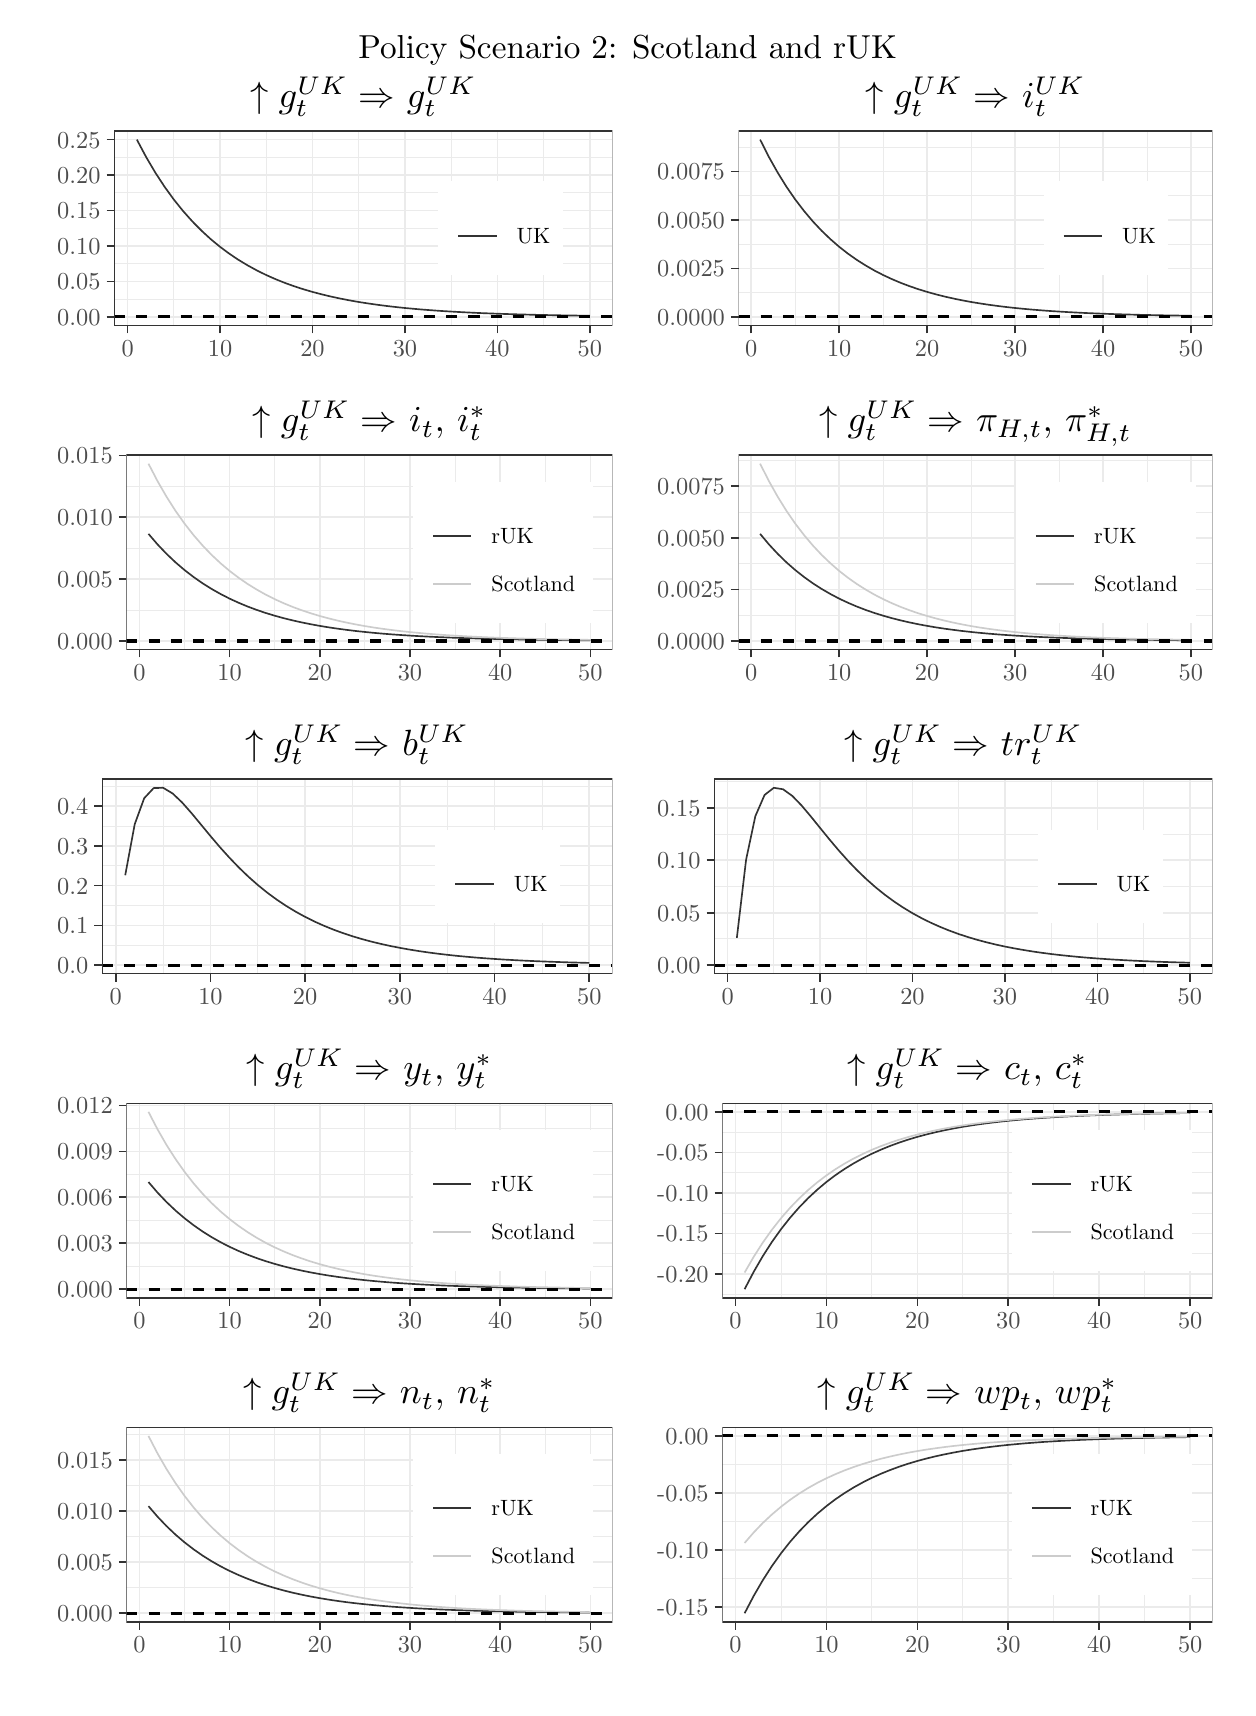
\begin{tikzpicture}[x=1pt,y=1pt]
\definecolor{fillColor}{RGB}{255,255,255}
\path[use as bounding box,fill=fillColor,fill opacity=0.00] (0,0) rectangle (433.62,599.84);
\begin{scope}
\path[clip] (  0.00,468.44) rectangle (216.81,585.55);
\definecolor{drawColor}{RGB}{255,255,255}
\definecolor{fillColor}{RGB}{255,255,255}

\path[draw=drawColor,line width= 0.6pt,line join=round,line cap=round,fill=fillColor] (  0.00,468.44) rectangle (216.81,585.55);
\end{scope}
\begin{scope}
\path[clip] ( 31.27,492.12) rectangle (211.31,562.59);
\definecolor{fillColor}{RGB}{255,255,255}

\path[fill=fillColor] ( 31.27,492.12) rectangle (211.31,562.59);
\definecolor{drawColor}{gray}{0.92}

\path[draw=drawColor,line width= 0.3pt,line join=round] ( 31.27,501.73) --
	(211.31,501.73);

\path[draw=drawColor,line width= 0.3pt,line join=round] ( 31.27,514.54) --
	(211.31,514.54);

\path[draw=drawColor,line width= 0.3pt,line join=round] ( 31.27,527.36) --
	(211.31,527.36);

\path[draw=drawColor,line width= 0.3pt,line join=round] ( 31.27,540.17) --
	(211.31,540.17);

\path[draw=drawColor,line width= 0.3pt,line join=round] ( 31.27,552.98) --
	(211.31,552.98);

\path[draw=drawColor,line width= 0.3pt,line join=round] ( 52.81,492.12) --
	( 52.81,562.59);

\path[draw=drawColor,line width= 0.3pt,line join=round] ( 86.22,492.12) --
	( 86.22,562.59);

\path[draw=drawColor,line width= 0.3pt,line join=round] (119.62,492.12) --
	(119.62,562.59);

\path[draw=drawColor,line width= 0.3pt,line join=round] (153.02,492.12) --
	(153.02,562.59);

\path[draw=drawColor,line width= 0.3pt,line join=round] (186.43,492.12) --
	(186.43,562.59);

\path[draw=drawColor,line width= 0.6pt,line join=round] ( 31.27,495.32) --
	(211.31,495.32);

\path[draw=drawColor,line width= 0.6pt,line join=round] ( 31.27,508.14) --
	(211.31,508.14);

\path[draw=drawColor,line width= 0.6pt,line join=round] ( 31.27,520.95) --
	(211.31,520.95);

\path[draw=drawColor,line width= 0.6pt,line join=round] ( 31.27,533.76) --
	(211.31,533.76);

\path[draw=drawColor,line width= 0.6pt,line join=round] ( 31.27,546.58) --
	(211.31,546.58);

\path[draw=drawColor,line width= 0.6pt,line join=round] ( 31.27,559.39) --
	(211.31,559.39);

\path[draw=drawColor,line width= 0.6pt,line join=round] ( 36.11,492.12) --
	( 36.11,562.59);

\path[draw=drawColor,line width= 0.6pt,line join=round] ( 69.52,492.12) --
	( 69.52,562.59);

\path[draw=drawColor,line width= 0.6pt,line join=round] (102.92,492.12) --
	(102.92,562.59);

\path[draw=drawColor,line width= 0.6pt,line join=round] (136.32,492.12) --
	(136.32,562.59);

\path[draw=drawColor,line width= 0.6pt,line join=round] (169.72,492.12) --
	(169.72,562.59);

\path[draw=drawColor,line width= 0.6pt,line join=round] (203.13,492.12) --
	(203.13,562.59);
\definecolor{drawColor}{gray}{0.20}

\path[draw=drawColor,line width= 0.6pt,line join=round] ( 39.45,559.39) --
	( 42.79,553.11) --
	( 46.13,547.45) --
	( 49.47,542.34) --
	( 52.81,537.73) --
	( 56.15,533.58) --
	( 59.50,529.83) --
	( 62.84,526.45) --
	( 66.18,523.39) --
	( 69.52,520.64) --
	( 72.86,518.16) --
	( 76.20,515.92) --
	( 79.54,513.91) --
	( 82.88,512.08) --
	( 86.22,510.44) --
	( 89.56,508.96) --
	( 92.90,507.62) --
	( 96.24,506.42) --
	( 99.58,505.33) --
	(102.92,504.35) --
	(106.26,503.47) --
	(109.60,502.67) --
	(112.94,501.95) --
	(116.28,501.30) --
	(119.62,500.71) --
	(122.96,500.19) --
	(126.30,499.71) --
	(129.64,499.28) --
	(132.98,498.89) --
	(136.32,498.54) --
	(139.66,498.23) --
	(143.00,497.94) --
	(146.34,497.69) --
	(149.68,497.45) --
	(153.02,497.25) --
	(156.36,497.06) --
	(159.70,496.89) --
	(163.04,496.73) --
	(166.38,496.60) --
	(169.72,496.47) --
	(173.06,496.36) --
	(176.40,496.26) --
	(179.74,496.17) --
	(183.08,496.08) --
	(186.43,496.01) --
	(189.77,495.94) --
	(193.11,495.88) --
	(196.45,495.83) --
	(199.79,495.78) --
	(203.13,495.73);
\definecolor{drawColor}{RGB}{0,0,0}

\path[draw=drawColor,line width= 1.1pt,dash pattern=on 4pt off 4pt ,line join=round] ( 31.27,495.32) -- (211.31,495.32);
\definecolor{drawColor}{gray}{0.20}

\path[draw=drawColor,line width= 0.6pt,line join=round,line cap=round] ( 31.27,492.12) rectangle (211.31,562.59);
\end{scope}
\begin{scope}
\path[clip] (  0.00,  0.00) rectangle (433.62,599.84);
\definecolor{drawColor}{gray}{0.30}

\node[text=drawColor,anchor=base east,inner sep=0pt, outer sep=0pt, scale=  0.88] at ( 26.32,492.29) {0.00};

\node[text=drawColor,anchor=base east,inner sep=0pt, outer sep=0pt, scale=  0.88] at ( 26.32,505.11) {0.05};

\node[text=drawColor,anchor=base east,inner sep=0pt, outer sep=0pt, scale=  0.88] at ( 26.32,517.92) {0.10};

\node[text=drawColor,anchor=base east,inner sep=0pt, outer sep=0pt, scale=  0.88] at ( 26.32,530.73) {0.15};

\node[text=drawColor,anchor=base east,inner sep=0pt, outer sep=0pt, scale=  0.88] at ( 26.32,543.55) {0.20};

\node[text=drawColor,anchor=base east,inner sep=0pt, outer sep=0pt, scale=  0.88] at ( 26.32,556.36) {0.25};
\end{scope}
\begin{scope}
\path[clip] (  0.00,  0.00) rectangle (433.62,599.84);
\definecolor{drawColor}{gray}{0.20}

\path[draw=drawColor,line width= 0.6pt,line join=round] ( 28.52,495.32) --
	( 31.27,495.32);

\path[draw=drawColor,line width= 0.6pt,line join=round] ( 28.52,508.14) --
	( 31.27,508.14);

\path[draw=drawColor,line width= 0.6pt,line join=round] ( 28.52,520.95) --
	( 31.27,520.95);

\path[draw=drawColor,line width= 0.6pt,line join=round] ( 28.52,533.76) --
	( 31.27,533.76);

\path[draw=drawColor,line width= 0.6pt,line join=round] ( 28.52,546.58) --
	( 31.27,546.58);

\path[draw=drawColor,line width= 0.6pt,line join=round] ( 28.52,559.39) --
	( 31.27,559.39);
\end{scope}
\begin{scope}
\path[clip] (  0.00,  0.00) rectangle (433.62,599.84);
\definecolor{drawColor}{gray}{0.20}

\path[draw=drawColor,line width= 0.6pt,line join=round] ( 36.11,489.37) --
	( 36.11,492.12);

\path[draw=drawColor,line width= 0.6pt,line join=round] ( 69.52,489.37) --
	( 69.52,492.12);

\path[draw=drawColor,line width= 0.6pt,line join=round] (102.92,489.37) --
	(102.92,492.12);

\path[draw=drawColor,line width= 0.6pt,line join=round] (136.32,489.37) --
	(136.32,492.12);

\path[draw=drawColor,line width= 0.6pt,line join=round] (169.72,489.37) --
	(169.72,492.12);

\path[draw=drawColor,line width= 0.6pt,line join=round] (203.13,489.37) --
	(203.13,492.12);
\end{scope}
\begin{scope}
\path[clip] (  0.00,  0.00) rectangle (433.62,599.84);
\definecolor{drawColor}{gray}{0.30}

\node[text=drawColor,anchor=base,inner sep=0pt, outer sep=0pt, scale=  0.88] at ( 36.11,481.11) {0};

\node[text=drawColor,anchor=base,inner sep=0pt, outer sep=0pt, scale=  0.88] at ( 69.52,481.11) {10};

\node[text=drawColor,anchor=base,inner sep=0pt, outer sep=0pt, scale=  0.88] at (102.92,481.11) {20};

\node[text=drawColor,anchor=base,inner sep=0pt, outer sep=0pt, scale=  0.88] at (136.32,481.11) {30};

\node[text=drawColor,anchor=base,inner sep=0pt, outer sep=0pt, scale=  0.88] at (169.72,481.11) {40};

\node[text=drawColor,anchor=base,inner sep=0pt, outer sep=0pt, scale=  0.88] at (203.13,481.11) {50};
\end{scope}
\begin{scope}
\path[clip] (  0.00,  0.00) rectangle (433.62,599.84);
\definecolor{fillColor}{RGB}{255,255,255}

\path[fill=fillColor] (148.30,510.43) rectangle (193.30,544.28);
\end{scope}
\begin{scope}
\path[clip] (  0.00,  0.00) rectangle (433.62,599.84);
\definecolor{fillColor}{RGB}{255,255,255}

\path[fill=fillColor] (153.80,515.93) rectangle (171.15,533.28);
\end{scope}
\begin{scope}
\path[clip] (  0.00,  0.00) rectangle (433.62,599.84);
\definecolor{drawColor}{gray}{0.20}

\path[draw=drawColor,line width= 0.6pt,line join=round] (155.54,524.61) -- (169.41,524.61);
\end{scope}
\begin{scope}
\path[clip] (  0.00,  0.00) rectangle (433.62,599.84);
\definecolor{drawColor}{RGB}{0,0,0}

\node[text=drawColor,anchor=base west,inner sep=0pt, outer sep=0pt, scale=  0.80] at (176.65,521.85) {UK};
\end{scope}
\begin{scope}
\path[clip] (  0.00,  0.00) rectangle (433.62,599.84);
\definecolor{drawColor}{RGB}{0,0,0}

\node[text=drawColor,anchor=base,inner sep=0pt, outer sep=0pt, scale=  1.32] at (121.29,570.96) {$\uparrow  g^{UK}_t \Rightarrow $ ${g^{UK}_t}$};
\end{scope}
\begin{scope}
\path[clip] (216.81,468.44) rectangle (433.62,585.55);
\definecolor{drawColor}{RGB}{255,255,255}
\definecolor{fillColor}{RGB}{255,255,255}

\path[draw=drawColor,line width= 0.6pt,line join=round,line cap=round,fill=fillColor] (216.81,468.44) rectangle (433.62,585.55);
\end{scope}
\begin{scope}
\path[clip] (256.88,492.12) rectangle (428.12,562.59);
\definecolor{fillColor}{RGB}{255,255,255}

\path[fill=fillColor] (256.88,492.12) rectangle (428.12,562.59);
\definecolor{drawColor}{gray}{0.92}

\path[draw=drawColor,line width= 0.3pt,line join=round] (256.88,504.08) --
	(428.12,504.08);

\path[draw=drawColor,line width= 0.3pt,line join=round] (256.88,521.59) --
	(428.12,521.59);

\path[draw=drawColor,line width= 0.3pt,line join=round] (256.88,539.10) --
	(428.12,539.10);

\path[draw=drawColor,line width= 0.3pt,line join=round] (256.88,556.61) --
	(428.12,556.61);

\path[draw=drawColor,line width= 0.3pt,line join=round] (277.37,492.12) --
	(277.37,562.59);

\path[draw=drawColor,line width= 0.3pt,line join=round] (309.14,492.12) --
	(309.14,562.59);

\path[draw=drawColor,line width= 0.3pt,line join=round] (340.91,492.12) --
	(340.91,562.59);

\path[draw=drawColor,line width= 0.3pt,line join=round] (372.68,492.12) --
	(372.68,562.59);

\path[draw=drawColor,line width= 0.3pt,line join=round] (404.45,492.12) --
	(404.45,562.59);

\path[draw=drawColor,line width= 0.6pt,line join=round] (256.88,495.32) --
	(428.12,495.32);

\path[draw=drawColor,line width= 0.6pt,line join=round] (256.88,512.83) --
	(428.12,512.83);

\path[draw=drawColor,line width= 0.6pt,line join=round] (256.88,530.35) --
	(428.12,530.35);

\path[draw=drawColor,line width= 0.6pt,line join=round] (256.88,547.86) --
	(428.12,547.86);

\path[draw=drawColor,line width= 0.6pt,line join=round] (261.48,492.12) --
	(261.48,562.59);

\path[draw=drawColor,line width= 0.6pt,line join=round] (293.25,492.12) --
	(293.25,562.59);

\path[draw=drawColor,line width= 0.6pt,line join=round] (325.03,492.12) --
	(325.03,562.59);

\path[draw=drawColor,line width= 0.6pt,line join=round] (356.80,492.12) --
	(356.80,562.59);

\path[draw=drawColor,line width= 0.6pt,line join=round] (388.57,492.12) --
	(388.57,562.59);

\path[draw=drawColor,line width= 0.6pt,line join=round] (420.34,492.12) --
	(420.34,562.59);
\definecolor{drawColor}{gray}{0.20}

\path[draw=drawColor,line width= 0.6pt,line join=round] (264.66,559.39) --
	(267.84,553.11) --
	(271.02,547.45) --
	(274.19,542.34) --
	(277.37,537.73) --
	(280.55,533.58) --
	(283.72,529.83) --
	(286.90,526.45) --
	(290.08,523.40) --
	(293.25,520.64) --
	(296.43,518.16) --
	(299.61,515.92) --
	(302.79,513.91) --
	(305.96,512.08) --
	(309.14,510.44) --
	(312.32,508.96) --
	(315.49,507.62) --
	(318.67,506.42) --
	(321.85,505.33) --
	(325.03,504.35) --
	(328.20,503.47) --
	(331.38,502.67) --
	(334.56,501.95) --
	(337.73,501.30) --
	(340.91,500.71) --
	(344.09,500.19) --
	(347.26,499.71) --
	(350.44,499.28) --
	(353.62,498.89) --
	(356.80,498.54) --
	(359.97,498.23) --
	(363.15,497.94) --
	(366.33,497.69) --
	(369.50,497.45) --
	(372.68,497.25) --
	(375.86,497.06) --
	(379.03,496.89) --
	(382.21,496.73) --
	(385.39,496.60) --
	(388.57,496.47) --
	(391.74,496.36) --
	(394.92,496.26) --
	(398.10,496.17) --
	(401.27,496.08) --
	(404.45,496.01) --
	(407.63,495.94) --
	(410.81,495.88) --
	(413.98,495.83) --
	(417.16,495.78) --
	(420.34,495.73);
\definecolor{drawColor}{RGB}{0,0,0}

\path[draw=drawColor,line width= 1.1pt,dash pattern=on 4pt off 4pt ,line join=round] (256.88,495.32) -- (428.12,495.32);
\definecolor{drawColor}{gray}{0.20}

\path[draw=drawColor,line width= 0.6pt,line join=round,line cap=round] (256.88,492.12) rectangle (428.12,562.59);
\end{scope}
\begin{scope}
\path[clip] (  0.00,  0.00) rectangle (433.62,599.84);
\definecolor{drawColor}{gray}{0.30}

\node[text=drawColor,anchor=base east,inner sep=0pt, outer sep=0pt, scale=  0.88] at (251.93,492.29) {0.0000};

\node[text=drawColor,anchor=base east,inner sep=0pt, outer sep=0pt, scale=  0.88] at (251.93,509.80) {0.0025};

\node[text=drawColor,anchor=base east,inner sep=0pt, outer sep=0pt, scale=  0.88] at (251.93,527.31) {0.0050};

\node[text=drawColor,anchor=base east,inner sep=0pt, outer sep=0pt, scale=  0.88] at (251.93,544.83) {0.0075};
\end{scope}
\begin{scope}
\path[clip] (  0.00,  0.00) rectangle (433.62,599.84);
\definecolor{drawColor}{gray}{0.20}

\path[draw=drawColor,line width= 0.6pt,line join=round] (254.13,495.32) --
	(256.88,495.32);

\path[draw=drawColor,line width= 0.6pt,line join=round] (254.13,512.83) --
	(256.88,512.83);

\path[draw=drawColor,line width= 0.6pt,line join=round] (254.13,530.35) --
	(256.88,530.35);

\path[draw=drawColor,line width= 0.6pt,line join=round] (254.13,547.86) --
	(256.88,547.86);
\end{scope}
\begin{scope}
\path[clip] (  0.00,  0.00) rectangle (433.62,599.84);
\definecolor{drawColor}{gray}{0.20}

\path[draw=drawColor,line width= 0.6pt,line join=round] (261.48,489.37) --
	(261.48,492.12);

\path[draw=drawColor,line width= 0.6pt,line join=round] (293.25,489.37) --
	(293.25,492.12);

\path[draw=drawColor,line width= 0.6pt,line join=round] (325.03,489.37) --
	(325.03,492.12);

\path[draw=drawColor,line width= 0.6pt,line join=round] (356.80,489.37) --
	(356.80,492.12);

\path[draw=drawColor,line width= 0.6pt,line join=round] (388.57,489.37) --
	(388.57,492.12);

\path[draw=drawColor,line width= 0.6pt,line join=round] (420.34,489.37) --
	(420.34,492.12);
\end{scope}
\begin{scope}
\path[clip] (  0.00,  0.00) rectangle (433.62,599.84);
\definecolor{drawColor}{gray}{0.30}

\node[text=drawColor,anchor=base,inner sep=0pt, outer sep=0pt, scale=  0.88] at (261.48,481.11) {0};

\node[text=drawColor,anchor=base,inner sep=0pt, outer sep=0pt, scale=  0.88] at (293.25,481.11) {10};

\node[text=drawColor,anchor=base,inner sep=0pt, outer sep=0pt, scale=  0.88] at (325.03,481.11) {20};

\node[text=drawColor,anchor=base,inner sep=0pt, outer sep=0pt, scale=  0.88] at (356.80,481.11) {30};

\node[text=drawColor,anchor=base,inner sep=0pt, outer sep=0pt, scale=  0.88] at (388.57,481.11) {40};

\node[text=drawColor,anchor=base,inner sep=0pt, outer sep=0pt, scale=  0.88] at (420.34,481.11) {50};
\end{scope}
\begin{scope}
\path[clip] (  0.00,  0.00) rectangle (433.62,599.84);
\definecolor{fillColor}{RGB}{255,255,255}

\path[fill=fillColor] (367.09,510.43) rectangle (412.09,544.28);
\end{scope}
\begin{scope}
\path[clip] (  0.00,  0.00) rectangle (433.62,599.84);
\definecolor{fillColor}{RGB}{255,255,255}

\path[fill=fillColor] (372.59,515.93) rectangle (389.94,533.28);
\end{scope}
\begin{scope}
\path[clip] (  0.00,  0.00) rectangle (433.62,599.84);
\definecolor{drawColor}{gray}{0.20}

\path[draw=drawColor,line width= 0.6pt,line join=round] (374.33,524.61) -- (388.20,524.61);
\end{scope}
\begin{scope}
\path[clip] (  0.00,  0.00) rectangle (433.62,599.84);
\definecolor{drawColor}{RGB}{0,0,0}

\node[text=drawColor,anchor=base west,inner sep=0pt, outer sep=0pt, scale=  0.80] at (395.44,521.85) {UK};
\end{scope}
\begin{scope}
\path[clip] (  0.00,  0.00) rectangle (433.62,599.84);
\definecolor{drawColor}{RGB}{0,0,0}

\node[text=drawColor,anchor=base,inner sep=0pt, outer sep=0pt, scale=  1.32] at (342.50,570.96) {$\uparrow  g^{UK}_t \Rightarrow $ ${i^{UK}_t}$};
\end{scope}
\begin{scope}
\path[clip] (  0.00,351.33) rectangle (216.81,468.44);
\definecolor{drawColor}{RGB}{255,255,255}
\definecolor{fillColor}{RGB}{255,255,255}

\path[draw=drawColor,line width= 0.6pt,line join=round,line cap=round,fill=fillColor] (  0.00,351.33) rectangle (216.81,468.44);
\end{scope}
\begin{scope}
\path[clip] ( 35.67,375.01) rectangle (211.31,445.48);
\definecolor{fillColor}{RGB}{255,255,255}

\path[fill=fillColor] ( 35.67,375.01) rectangle (211.31,445.48);
\definecolor{drawColor}{gray}{0.92}

\path[draw=drawColor,line width= 0.3pt,line join=round] ( 35.67,389.39) --
	(211.31,389.39);

\path[draw=drawColor,line width= 0.3pt,line join=round] ( 35.67,411.75) --
	(211.31,411.75);

\path[draw=drawColor,line width= 0.3pt,line join=round] ( 35.67,434.11) --
	(211.31,434.11);

\path[draw=drawColor,line width= 0.3pt,line join=round] ( 56.69,375.01) --
	( 56.69,445.48);

\path[draw=drawColor,line width= 0.3pt,line join=round] ( 89.27,375.01) --
	( 89.27,445.48);

\path[draw=drawColor,line width= 0.3pt,line join=round] (121.86,375.01) --
	(121.86,445.48);

\path[draw=drawColor,line width= 0.3pt,line join=round] (154.45,375.01) --
	(154.45,445.48);

\path[draw=drawColor,line width= 0.3pt,line join=round] (187.03,375.01) --
	(187.03,445.48);

\path[draw=drawColor,line width= 0.6pt,line join=round] ( 35.67,378.21) --
	(211.31,378.21);

\path[draw=drawColor,line width= 0.6pt,line join=round] ( 35.67,400.57) --
	(211.31,400.57);

\path[draw=drawColor,line width= 0.6pt,line join=round] ( 35.67,422.93) --
	(211.31,422.93);

\path[draw=drawColor,line width= 0.6pt,line join=round] ( 35.67,445.29) --
	(211.31,445.29);

\path[draw=drawColor,line width= 0.6pt,line join=round] ( 40.39,375.01) --
	( 40.39,445.48);

\path[draw=drawColor,line width= 0.6pt,line join=round] ( 72.98,375.01) --
	( 72.98,445.48);

\path[draw=drawColor,line width= 0.6pt,line join=round] (105.57,375.01) --
	(105.57,445.48);

\path[draw=drawColor,line width= 0.6pt,line join=round] (138.15,375.01) --
	(138.15,445.48);

\path[draw=drawColor,line width= 0.6pt,line join=round] (170.74,375.01) --
	(170.74,445.48);

\path[draw=drawColor,line width= 0.6pt,line join=round] (203.33,375.01) --
	(203.33,445.48);
\definecolor{drawColor}{gray}{0.20}

\path[draw=drawColor,line width= 0.6pt,line join=round] ( 43.65,416.93) --
	( 46.91,413.13) --
	( 50.17,409.71) --
	( 53.43,406.62) --
	( 56.69,403.84) --
	( 59.95,401.33) --
	( 63.20,399.06) --
	( 66.46,397.02) --
	( 69.72,395.18) --
	( 72.98,393.51) --
	( 76.24,392.02) --
	( 79.50,390.66) --
	( 82.76,389.44) --
	( 86.01,388.34) --
	( 89.27,387.35) --
	( 92.53,386.45) --
	( 95.79,385.65) --
	( 99.05,384.92) --
	(102.31,384.26) --
	(105.57,383.67) --
	(108.83,383.13) --
	(112.08,382.65) --
	(115.34,382.22) --
	(118.60,381.82) --
	(121.86,381.47) --
	(125.12,381.15) --
	(128.38,380.86) --
	(131.64,380.60) --
	(134.89,380.37) --
	(138.15,380.16) --
	(141.41,379.97) --
	(144.67,379.80) --
	(147.93,379.64) --
	(151.19,379.50) --
	(154.45,379.37) --
	(157.71,379.26) --
	(160.96,379.16) --
	(164.22,379.07) --
	(167.48,378.98) --
	(170.74,378.91) --
	(174.00,378.84) --
	(177.26,378.78) --
	(180.52,378.72) --
	(183.77,378.67) --
	(187.03,378.63) --
	(190.29,378.59) --
	(193.55,378.55) --
	(196.81,378.52) --
	(200.07,378.49) --
	(203.33,378.46);
\definecolor{drawColor}{gray}{0.80}

\path[draw=drawColor,line width= 0.6pt,line join=round] ( 43.65,442.28) --
	( 46.91,436.00) --
	( 50.17,430.34) --
	( 53.43,425.23) --
	( 56.69,420.62) --
	( 59.95,416.46) --
	( 63.20,412.72) --
	( 66.46,409.33) --
	( 69.72,406.28) --
	( 72.98,403.53) --
	( 76.24,401.05) --
	( 79.50,398.81) --
	( 82.76,396.80) --
	( 86.01,394.97) --
	( 89.27,393.33) --
	( 92.53,391.85) --
	( 95.79,390.51) --
	( 99.05,389.31) --
	(102.31,388.22) --
	(105.57,387.24) --
	(108.83,386.36) --
	(112.08,385.56) --
	(115.34,384.84) --
	(118.60,384.19) --
	(121.86,383.60) --
	(125.12,383.07) --
	(128.38,382.60) --
	(131.64,382.17) --
	(134.89,381.78) --
	(138.15,381.43) --
	(141.41,381.12) --
	(144.67,380.83) --
	(147.93,380.57) --
	(151.19,380.34) --
	(154.45,380.13) --
	(157.71,379.95) --
	(160.96,379.78) --
	(164.22,379.62) --
	(167.48,379.48) --
	(170.74,379.36) --
	(174.00,379.25) --
	(177.26,379.15) --
	(180.52,379.05) --
	(183.77,378.97) --
	(187.03,378.90) --
	(190.29,378.83) --
	(193.55,378.77) --
	(196.81,378.72) --
	(200.07,378.67) --
	(203.33,378.62);
\definecolor{drawColor}{RGB}{0,0,0}

\path[draw=drawColor,line width= 1.1pt,dash pattern=on 4pt off 4pt ,line join=round] ( 35.67,378.21) -- (211.31,378.21);
\definecolor{drawColor}{gray}{0.20}

\path[draw=drawColor,line width= 0.6pt,line join=round,line cap=round] ( 35.67,375.01) rectangle (211.31,445.48);
\end{scope}
\begin{scope}
\path[clip] (  0.00,  0.00) rectangle (433.62,599.84);
\definecolor{drawColor}{gray}{0.30}

\node[text=drawColor,anchor=base east,inner sep=0pt, outer sep=0pt, scale=  0.88] at ( 30.72,375.18) {0.000};

\node[text=drawColor,anchor=base east,inner sep=0pt, outer sep=0pt, scale=  0.88] at ( 30.72,397.54) {0.005};

\node[text=drawColor,anchor=base east,inner sep=0pt, outer sep=0pt, scale=  0.88] at ( 30.72,419.90) {0.010};

\node[text=drawColor,anchor=base east,inner sep=0pt, outer sep=0pt, scale=  0.88] at ( 30.72,442.26) {0.015};
\end{scope}
\begin{scope}
\path[clip] (  0.00,  0.00) rectangle (433.62,599.84);
\definecolor{drawColor}{gray}{0.20}

\path[draw=drawColor,line width= 0.6pt,line join=round] ( 32.92,378.21) --
	( 35.67,378.21);

\path[draw=drawColor,line width= 0.6pt,line join=round] ( 32.92,400.57) --
	( 35.67,400.57);

\path[draw=drawColor,line width= 0.6pt,line join=round] ( 32.92,422.93) --
	( 35.67,422.93);

\path[draw=drawColor,line width= 0.6pt,line join=round] ( 32.92,445.29) --
	( 35.67,445.29);
\end{scope}
\begin{scope}
\path[clip] (  0.00,  0.00) rectangle (433.62,599.84);
\definecolor{drawColor}{gray}{0.20}

\path[draw=drawColor,line width= 0.6pt,line join=round] ( 40.39,372.26) --
	( 40.39,375.01);

\path[draw=drawColor,line width= 0.6pt,line join=round] ( 72.98,372.26) --
	( 72.98,375.01);

\path[draw=drawColor,line width= 0.6pt,line join=round] (105.57,372.26) --
	(105.57,375.01);

\path[draw=drawColor,line width= 0.6pt,line join=round] (138.15,372.26) --
	(138.15,375.01);

\path[draw=drawColor,line width= 0.6pt,line join=round] (170.74,372.26) --
	(170.74,375.01);

\path[draw=drawColor,line width= 0.6pt,line join=round] (203.33,372.26) --
	(203.33,375.01);
\end{scope}
\begin{scope}
\path[clip] (  0.00,  0.00) rectangle (433.62,599.84);
\definecolor{drawColor}{gray}{0.30}

\node[text=drawColor,anchor=base,inner sep=0pt, outer sep=0pt, scale=  0.88] at ( 40.39,364.00) {0};

\node[text=drawColor,anchor=base,inner sep=0pt, outer sep=0pt, scale=  0.88] at ( 72.98,364.00) {10};

\node[text=drawColor,anchor=base,inner sep=0pt, outer sep=0pt, scale=  0.88] at (105.57,364.00) {20};

\node[text=drawColor,anchor=base,inner sep=0pt, outer sep=0pt, scale=  0.88] at (138.15,364.00) {30};

\node[text=drawColor,anchor=base,inner sep=0pt, outer sep=0pt, scale=  0.88] at (170.74,364.00) {40};

\node[text=drawColor,anchor=base,inner sep=0pt, outer sep=0pt, scale=  0.88] at (203.33,364.00) {50};
\end{scope}
\begin{scope}
\path[clip] (  0.00,  0.00) rectangle (433.62,599.84);
\definecolor{fillColor}{RGB}{255,255,255}

\path[fill=fillColor] (139.25,384.65) rectangle (204.34,435.84);
\end{scope}
\begin{scope}
\path[clip] (  0.00,  0.00) rectangle (433.62,599.84);
\definecolor{fillColor}{RGB}{255,255,255}

\path[fill=fillColor] (144.75,407.50) rectangle (162.09,424.84);
\end{scope}
\begin{scope}
\path[clip] (  0.00,  0.00) rectangle (433.62,599.84);
\definecolor{drawColor}{gray}{0.20}

\path[draw=drawColor,line width= 0.6pt,line join=round] (146.48,416.17) -- (160.36,416.17);
\end{scope}
\begin{scope}
\path[clip] (  0.00,  0.00) rectangle (433.62,599.84);
\definecolor{fillColor}{RGB}{255,255,255}

\path[fill=fillColor] (144.75,390.15) rectangle (162.09,407.50);
\end{scope}
\begin{scope}
\path[clip] (  0.00,  0.00) rectangle (433.62,599.84);
\definecolor{drawColor}{gray}{0.80}

\path[draw=drawColor,line width= 0.6pt,line join=round] (146.48,398.82) -- (160.36,398.82);
\end{scope}
\begin{scope}
\path[clip] (  0.00,  0.00) rectangle (433.62,599.84);
\definecolor{drawColor}{RGB}{0,0,0}

\node[text=drawColor,anchor=base west,inner sep=0pt, outer sep=0pt, scale=  0.80] at (167.59,413.41) {rUK};
\end{scope}
\begin{scope}
\path[clip] (  0.00,  0.00) rectangle (433.62,599.84);
\definecolor{drawColor}{RGB}{0,0,0}

\node[text=drawColor,anchor=base west,inner sep=0pt, outer sep=0pt, scale=  0.80] at (167.59,396.07) {Scotland};
\end{scope}
\begin{scope}
\path[clip] (  0.00,  0.00) rectangle (433.62,599.84);
\definecolor{drawColor}{RGB}{0,0,0}

\node[text=drawColor,anchor=base,inner sep=0pt, outer sep=0pt, scale=  1.32] at (123.49,453.85) {$\uparrow  g^{UK}_t \Rightarrow $ ${i_t}$, ${i^*_t}$};
\end{scope}
\begin{scope}
\path[clip] (216.81,351.33) rectangle (433.62,468.44);
\definecolor{drawColor}{RGB}{255,255,255}
\definecolor{fillColor}{RGB}{255,255,255}

\path[draw=drawColor,line width= 0.6pt,line join=round,line cap=round,fill=fillColor] (216.81,351.33) rectangle (433.62,468.44);
\end{scope}
\begin{scope}
\path[clip] (256.88,375.01) rectangle (428.12,445.48);
\definecolor{fillColor}{RGB}{255,255,255}

\path[fill=fillColor] (256.88,375.01) rectangle (428.12,445.48);
\definecolor{drawColor}{gray}{0.92}

\path[draw=drawColor,line width= 0.3pt,line join=round] (256.88,387.54) --
	(428.12,387.54);

\path[draw=drawColor,line width= 0.3pt,line join=round] (256.88,406.19) --
	(428.12,406.19);

\path[draw=drawColor,line width= 0.3pt,line join=round] (256.88,424.85) --
	(428.12,424.85);

\path[draw=drawColor,line width= 0.3pt,line join=round] (256.88,443.50) --
	(428.12,443.50);

\path[draw=drawColor,line width= 0.3pt,line join=round] (277.37,375.01) --
	(277.37,445.48);

\path[draw=drawColor,line width= 0.3pt,line join=round] (309.14,375.01) --
	(309.14,445.48);

\path[draw=drawColor,line width= 0.3pt,line join=round] (340.91,375.01) --
	(340.91,445.48);

\path[draw=drawColor,line width= 0.3pt,line join=round] (372.68,375.01) --
	(372.68,445.48);

\path[draw=drawColor,line width= 0.3pt,line join=round] (404.45,375.01) --
	(404.45,445.48);

\path[draw=drawColor,line width= 0.6pt,line join=round] (256.88,378.21) --
	(428.12,378.21);

\path[draw=drawColor,line width= 0.6pt,line join=round] (256.88,396.87) --
	(428.12,396.87);

\path[draw=drawColor,line width= 0.6pt,line join=round] (256.88,415.52) --
	(428.12,415.52);

\path[draw=drawColor,line width= 0.6pt,line join=round] (256.88,434.18) --
	(428.12,434.18);

\path[draw=drawColor,line width= 0.6pt,line join=round] (261.48,375.01) --
	(261.48,445.48);

\path[draw=drawColor,line width= 0.6pt,line join=round] (293.25,375.01) --
	(293.25,445.48);

\path[draw=drawColor,line width= 0.6pt,line join=round] (325.03,375.01) --
	(325.03,445.48);

\path[draw=drawColor,line width= 0.6pt,line join=round] (356.80,375.01) --
	(356.80,445.48);

\path[draw=drawColor,line width= 0.6pt,line join=round] (388.57,375.01) --
	(388.57,445.48);

\path[draw=drawColor,line width= 0.6pt,line join=round] (420.34,375.01) --
	(420.34,445.48);
\definecolor{drawColor}{gray}{0.20}

\path[draw=drawColor,line width= 0.6pt,line join=round] (264.66,416.93) --
	(267.84,413.13) --
	(271.02,409.71) --
	(274.19,406.62) --
	(277.37,403.84) --
	(280.55,401.33) --
	(283.72,399.06) --
	(286.90,397.02) --
	(290.08,395.18) --
	(293.25,393.51) --
	(296.43,392.02) --
	(299.61,390.66) --
	(302.79,389.44) --
	(305.96,388.34) --
	(309.14,387.35) --
	(312.32,386.45) --
	(315.49,385.65) --
	(318.67,384.92) --
	(321.85,384.26) --
	(325.03,383.67) --
	(328.20,383.13) --
	(331.38,382.65) --
	(334.56,382.22) --
	(337.73,381.82) --
	(340.91,381.47) --
	(344.09,381.15) --
	(347.26,380.86) --
	(350.44,380.60) --
	(353.62,380.37) --
	(356.80,380.16) --
	(359.97,379.97) --
	(363.15,379.80) --
	(366.33,379.64) --
	(369.50,379.50) --
	(372.68,379.37) --
	(375.86,379.26) --
	(379.03,379.16) --
	(382.21,379.07) --
	(385.39,378.98) --
	(388.57,378.91) --
	(391.74,378.84) --
	(394.92,378.78) --
	(398.10,378.72) --
	(401.27,378.67) --
	(404.45,378.63) --
	(407.63,378.59) --
	(410.81,378.55) --
	(413.98,378.52) --
	(417.16,378.49) --
	(420.34,378.46);
\definecolor{drawColor}{gray}{0.80}

\path[draw=drawColor,line width= 0.6pt,line join=round] (264.66,442.28) --
	(267.84,436.00) --
	(271.02,430.34) --
	(274.19,425.23) --
	(277.37,420.62) --
	(280.55,416.47) --
	(283.72,412.72) --
	(286.90,409.33) --
	(290.08,406.29) --
	(293.25,403.53) --
	(296.43,401.05) --
	(299.61,398.81) --
	(302.79,396.80) --
	(305.96,394.97) --
	(309.14,393.33) --
	(312.32,391.85) --
	(315.49,390.51) --
	(318.67,389.31) --
	(321.85,388.22) --
	(325.03,387.24) --
	(328.20,386.36) --
	(331.38,385.56) --
	(334.56,384.84) --
	(337.73,384.19) --
	(340.91,383.60) --
	(344.09,383.07) --
	(347.26,382.60) --
	(350.44,382.17) --
	(353.62,381.78) --
	(356.80,381.43) --
	(359.97,381.12) --
	(363.15,380.83) --
	(366.33,380.57) --
	(369.50,380.34) --
	(372.68,380.13) --
	(375.86,379.95) --
	(379.03,379.78) --
	(382.21,379.62) --
	(385.39,379.48) --
	(388.57,379.36) --
	(391.74,379.25) --
	(394.92,379.15) --
	(398.10,379.05) --
	(401.27,378.97) --
	(404.45,378.90) --
	(407.63,378.83) --
	(410.81,378.77) --
	(413.98,378.72) --
	(417.16,378.67) --
	(420.34,378.62);
\definecolor{drawColor}{RGB}{0,0,0}

\path[draw=drawColor,line width= 1.1pt,dash pattern=on 4pt off 4pt ,line join=round] (256.88,378.21) -- (428.12,378.21);
\definecolor{drawColor}{gray}{0.20}

\path[draw=drawColor,line width= 0.6pt,line join=round,line cap=round] (256.88,375.01) rectangle (428.12,445.48);
\end{scope}
\begin{scope}
\path[clip] (  0.00,  0.00) rectangle (433.62,599.84);
\definecolor{drawColor}{gray}{0.30}

\node[text=drawColor,anchor=base east,inner sep=0pt, outer sep=0pt, scale=  0.88] at (251.93,375.18) {0.0000};

\node[text=drawColor,anchor=base east,inner sep=0pt, outer sep=0pt, scale=  0.88] at (251.93,393.84) {0.0025};

\node[text=drawColor,anchor=base east,inner sep=0pt, outer sep=0pt, scale=  0.88] at (251.93,412.49) {0.0050};

\node[text=drawColor,anchor=base east,inner sep=0pt, outer sep=0pt, scale=  0.88] at (251.93,431.14) {0.0075};
\end{scope}
\begin{scope}
\path[clip] (  0.00,  0.00) rectangle (433.62,599.84);
\definecolor{drawColor}{gray}{0.20}

\path[draw=drawColor,line width= 0.6pt,line join=round] (254.13,378.21) --
	(256.88,378.21);

\path[draw=drawColor,line width= 0.6pt,line join=round] (254.13,396.87) --
	(256.88,396.87);

\path[draw=drawColor,line width= 0.6pt,line join=round] (254.13,415.52) --
	(256.88,415.52);

\path[draw=drawColor,line width= 0.6pt,line join=round] (254.13,434.18) --
	(256.88,434.18);
\end{scope}
\begin{scope}
\path[clip] (  0.00,  0.00) rectangle (433.62,599.84);
\definecolor{drawColor}{gray}{0.20}

\path[draw=drawColor,line width= 0.6pt,line join=round] (261.48,372.26) --
	(261.48,375.01);

\path[draw=drawColor,line width= 0.6pt,line join=round] (293.25,372.26) --
	(293.25,375.01);

\path[draw=drawColor,line width= 0.6pt,line join=round] (325.03,372.26) --
	(325.03,375.01);

\path[draw=drawColor,line width= 0.6pt,line join=round] (356.80,372.26) --
	(356.80,375.01);

\path[draw=drawColor,line width= 0.6pt,line join=round] (388.57,372.26) --
	(388.57,375.01);

\path[draw=drawColor,line width= 0.6pt,line join=round] (420.34,372.26) --
	(420.34,375.01);
\end{scope}
\begin{scope}
\path[clip] (  0.00,  0.00) rectangle (433.62,599.84);
\definecolor{drawColor}{gray}{0.30}

\node[text=drawColor,anchor=base,inner sep=0pt, outer sep=0pt, scale=  0.88] at (261.48,364.00) {0};

\node[text=drawColor,anchor=base,inner sep=0pt, outer sep=0pt, scale=  0.88] at (293.25,364.00) {10};

\node[text=drawColor,anchor=base,inner sep=0pt, outer sep=0pt, scale=  0.88] at (325.03,364.00) {20};

\node[text=drawColor,anchor=base,inner sep=0pt, outer sep=0pt, scale=  0.88] at (356.80,364.00) {30};

\node[text=drawColor,anchor=base,inner sep=0pt, outer sep=0pt, scale=  0.88] at (388.57,364.00) {40};

\node[text=drawColor,anchor=base,inner sep=0pt, outer sep=0pt, scale=  0.88] at (420.34,364.00) {50};
\end{scope}
\begin{scope}
\path[clip] (  0.00,  0.00) rectangle (433.62,599.84);
\definecolor{fillColor}{RGB}{255,255,255}

\path[fill=fillColor] (357.05,384.65) rectangle (422.14,435.84);
\end{scope}
\begin{scope}
\path[clip] (  0.00,  0.00) rectangle (433.62,599.84);
\definecolor{fillColor}{RGB}{255,255,255}

\path[fill=fillColor] (362.55,407.50) rectangle (379.89,424.84);
\end{scope}
\begin{scope}
\path[clip] (  0.00,  0.00) rectangle (433.62,599.84);
\definecolor{drawColor}{gray}{0.20}

\path[draw=drawColor,line width= 0.6pt,line join=round] (364.28,416.17) -- (378.16,416.17);
\end{scope}
\begin{scope}
\path[clip] (  0.00,  0.00) rectangle (433.62,599.84);
\definecolor{fillColor}{RGB}{255,255,255}

\path[fill=fillColor] (362.55,390.15) rectangle (379.89,407.50);
\end{scope}
\begin{scope}
\path[clip] (  0.00,  0.00) rectangle (433.62,599.84);
\definecolor{drawColor}{gray}{0.80}

\path[draw=drawColor,line width= 0.6pt,line join=round] (364.28,398.82) -- (378.16,398.82);
\end{scope}
\begin{scope}
\path[clip] (  0.00,  0.00) rectangle (433.62,599.84);
\definecolor{drawColor}{RGB}{0,0,0}

\node[text=drawColor,anchor=base west,inner sep=0pt, outer sep=0pt, scale=  0.80] at (385.39,413.41) {rUK};
\end{scope}
\begin{scope}
\path[clip] (  0.00,  0.00) rectangle (433.62,599.84);
\definecolor{drawColor}{RGB}{0,0,0}

\node[text=drawColor,anchor=base west,inner sep=0pt, outer sep=0pt, scale=  0.80] at (385.39,396.07) {Scotland};
\end{scope}
\begin{scope}
\path[clip] (  0.00,  0.00) rectangle (433.62,599.84);
\definecolor{drawColor}{RGB}{0,0,0}

\node[text=drawColor,anchor=base,inner sep=0pt, outer sep=0pt, scale=  1.32] at (342.50,453.85) {$\uparrow  g^{UK}_t \Rightarrow $ ${\pi_{H,t}}$, ${\pi^*_{H,t}}$};
\end{scope}
\begin{scope}
\path[clip] (  0.00,234.22) rectangle (216.81,351.33);
\definecolor{drawColor}{RGB}{255,255,255}
\definecolor{fillColor}{RGB}{255,255,255}

\path[draw=drawColor,line width= 0.6pt,line join=round,line cap=round,fill=fillColor] (  0.00,234.22) rectangle (216.81,351.33);
\end{scope}
\begin{scope}
\path[clip] ( 26.87,257.90) rectangle (211.31,328.37);
\definecolor{fillColor}{RGB}{255,255,255}

\path[fill=fillColor] ( 26.87,257.90) rectangle (211.31,328.37);
\definecolor{drawColor}{gray}{0.92}

\path[draw=drawColor,line width= 0.3pt,line join=round] ( 26.87,268.28) --
	(211.31,268.28);

\path[draw=drawColor,line width= 0.3pt,line join=round] ( 26.87,282.62) --
	(211.31,282.62);

\path[draw=drawColor,line width= 0.3pt,line join=round] ( 26.87,296.97) --
	(211.31,296.97);

\path[draw=drawColor,line width= 0.3pt,line join=round] ( 26.87,311.32) --
	(211.31,311.32);

\path[draw=drawColor,line width= 0.3pt,line join=round] ( 26.87,325.67) --
	(211.31,325.67);

\path[draw=drawColor,line width= 0.3pt,line join=round] ( 48.94,257.90) --
	( 48.94,328.37);

\path[draw=drawColor,line width= 0.3pt,line join=round] ( 83.16,257.90) --
	( 83.16,328.37);

\path[draw=drawColor,line width= 0.3pt,line join=round] (117.38,257.90) --
	(117.38,328.37);

\path[draw=drawColor,line width= 0.3pt,line join=round] (151.60,257.90) --
	(151.60,328.37);

\path[draw=drawColor,line width= 0.3pt,line join=round] (185.82,257.90) --
	(185.82,328.37);

\path[draw=drawColor,line width= 0.6pt,line join=round] ( 26.87,261.10) --
	(211.31,261.10);

\path[draw=drawColor,line width= 0.6pt,line join=round] ( 26.87,275.45) --
	(211.31,275.45);

\path[draw=drawColor,line width= 0.6pt,line join=round] ( 26.87,289.80) --
	(211.31,289.80);

\path[draw=drawColor,line width= 0.6pt,line join=round] ( 26.87,304.15) --
	(211.31,304.15);

\path[draw=drawColor,line width= 0.6pt,line join=round] ( 26.87,318.50) --
	(211.31,318.50);

\path[draw=drawColor,line width= 0.6pt,line join=round] ( 31.83,257.90) --
	( 31.83,328.37);

\path[draw=drawColor,line width= 0.6pt,line join=round] ( 66.05,257.90) --
	( 66.05,328.37);

\path[draw=drawColor,line width= 0.6pt,line join=round] (100.27,257.90) --
	(100.27,328.37);

\path[draw=drawColor,line width= 0.6pt,line join=round] (134.49,257.90) --
	(134.49,328.37);

\path[draw=drawColor,line width= 0.6pt,line join=round] (168.71,257.90) --
	(168.71,328.37);

\path[draw=drawColor,line width= 0.6pt,line join=round] (202.93,257.90) --
	(202.93,328.37);
\definecolor{drawColor}{gray}{0.20}

\path[draw=drawColor,line width= 0.6pt,line join=round] ( 35.25,293.57) --
	( 38.68,312.00) --
	( 42.10,321.39) --
	( 45.52,325.06) --
	( 48.94,325.17) --
	( 52.36,323.13) --
	( 55.79,319.88) --
	( 59.21,316.00) --
	( 62.63,311.87) --
	( 66.05,307.73) --
	( 69.47,303.71) --
	( 72.90,299.91) --
	( 76.32,296.35) --
	( 79.74,293.06) --
	( 83.16,290.04) --
	( 86.58,287.27) --
	( 90.00,284.76) --
	( 93.43,282.47) --
	( 96.85,280.40) --
	(100.27,278.52) --
	(103.69,276.82) --
	(107.11,275.29) --
	(110.54,273.90) --
	(113.96,272.65) --
	(117.38,271.52) --
	(120.80,270.50) --
	(124.22,269.58) --
	(127.65,268.75) --
	(131.07,268.00) --
	(134.49,267.33) --
	(137.91,266.72) --
	(141.33,266.17) --
	(144.75,265.67) --
	(148.18,265.22) --
	(151.60,264.82) --
	(155.02,264.45) --
	(158.44,264.13) --
	(161.86,263.83) --
	(165.29,263.56) --
	(168.71,263.32) --
	(172.13,263.10) --
	(175.55,262.91) --
	(178.97,262.73) --
	(182.40,262.57) --
	(185.82,262.43) --
	(189.24,262.30) --
	(192.66,262.18) --
	(196.08,262.07) --
	(199.50,261.98) --
	(202.93,261.89);
\definecolor{drawColor}{RGB}{0,0,0}

\path[draw=drawColor,line width= 1.1pt,dash pattern=on 4pt off 4pt ,line join=round] ( 26.87,261.10) -- (211.31,261.10);
\definecolor{drawColor}{gray}{0.20}

\path[draw=drawColor,line width= 0.6pt,line join=round,line cap=round] ( 26.87,257.90) rectangle (211.31,328.37);
\end{scope}
\begin{scope}
\path[clip] (  0.00,  0.00) rectangle (433.62,599.84);
\definecolor{drawColor}{gray}{0.30}

\node[text=drawColor,anchor=base east,inner sep=0pt, outer sep=0pt, scale=  0.88] at ( 21.92,258.07) {0.0};

\node[text=drawColor,anchor=base east,inner sep=0pt, outer sep=0pt, scale=  0.88] at ( 21.92,272.42) {0.1};

\node[text=drawColor,anchor=base east,inner sep=0pt, outer sep=0pt, scale=  0.88] at ( 21.92,286.77) {0.2};

\node[text=drawColor,anchor=base east,inner sep=0pt, outer sep=0pt, scale=  0.88] at ( 21.92,301.12) {0.3};

\node[text=drawColor,anchor=base east,inner sep=0pt, outer sep=0pt, scale=  0.88] at ( 21.92,315.47) {0.4};
\end{scope}
\begin{scope}
\path[clip] (  0.00,  0.00) rectangle (433.62,599.84);
\definecolor{drawColor}{gray}{0.20}

\path[draw=drawColor,line width= 0.6pt,line join=round] ( 24.12,261.10) --
	( 26.87,261.10);

\path[draw=drawColor,line width= 0.6pt,line join=round] ( 24.12,275.45) --
	( 26.87,275.45);

\path[draw=drawColor,line width= 0.6pt,line join=round] ( 24.12,289.80) --
	( 26.87,289.80);

\path[draw=drawColor,line width= 0.6pt,line join=round] ( 24.12,304.15) --
	( 26.87,304.15);

\path[draw=drawColor,line width= 0.6pt,line join=round] ( 24.12,318.50) --
	( 26.87,318.50);
\end{scope}
\begin{scope}
\path[clip] (  0.00,  0.00) rectangle (433.62,599.84);
\definecolor{drawColor}{gray}{0.20}

\path[draw=drawColor,line width= 0.6pt,line join=round] ( 31.83,255.15) --
	( 31.83,257.90);

\path[draw=drawColor,line width= 0.6pt,line join=round] ( 66.05,255.15) --
	( 66.05,257.90);

\path[draw=drawColor,line width= 0.6pt,line join=round] (100.27,255.15) --
	(100.27,257.90);

\path[draw=drawColor,line width= 0.6pt,line join=round] (134.49,255.15) --
	(134.49,257.90);

\path[draw=drawColor,line width= 0.6pt,line join=round] (168.71,255.15) --
	(168.71,257.90);

\path[draw=drawColor,line width= 0.6pt,line join=round] (202.93,255.15) --
	(202.93,257.90);
\end{scope}
\begin{scope}
\path[clip] (  0.00,  0.00) rectangle (433.62,599.84);
\definecolor{drawColor}{gray}{0.30}

\node[text=drawColor,anchor=base,inner sep=0pt, outer sep=0pt, scale=  0.88] at ( 31.83,246.89) {0};

\node[text=drawColor,anchor=base,inner sep=0pt, outer sep=0pt, scale=  0.88] at ( 66.05,246.89) {10};

\node[text=drawColor,anchor=base,inner sep=0pt, outer sep=0pt, scale=  0.88] at (100.27,246.89) {20};

\node[text=drawColor,anchor=base,inner sep=0pt, outer sep=0pt, scale=  0.88] at (134.49,246.89) {30};

\node[text=drawColor,anchor=base,inner sep=0pt, outer sep=0pt, scale=  0.88] at (168.71,246.89) {40};

\node[text=drawColor,anchor=base,inner sep=0pt, outer sep=0pt, scale=  0.88] at (202.93,246.89) {50};
\end{scope}
\begin{scope}
\path[clip] (  0.00,  0.00) rectangle (433.62,599.84);
\definecolor{fillColor}{RGB}{255,255,255}

\path[fill=fillColor] (147.31,276.21) rectangle (192.31,310.06);
\end{scope}
\begin{scope}
\path[clip] (  0.00,  0.00) rectangle (433.62,599.84);
\definecolor{fillColor}{RGB}{255,255,255}

\path[fill=fillColor] (152.81,281.71) rectangle (170.16,299.06);
\end{scope}
\begin{scope}
\path[clip] (  0.00,  0.00) rectangle (433.62,599.84);
\definecolor{drawColor}{gray}{0.20}

\path[draw=drawColor,line width= 0.6pt,line join=round] (154.55,290.38) -- (168.42,290.38);
\end{scope}
\begin{scope}
\path[clip] (  0.00,  0.00) rectangle (433.62,599.84);
\definecolor{drawColor}{RGB}{0,0,0}

\node[text=drawColor,anchor=base west,inner sep=0pt, outer sep=0pt, scale=  0.80] at (175.66,287.63) {UK};
\end{scope}
\begin{scope}
\path[clip] (  0.00,  0.00) rectangle (433.62,599.84);
\definecolor{drawColor}{RGB}{0,0,0}

\node[text=drawColor,anchor=base,inner sep=0pt, outer sep=0pt, scale=  1.32] at (119.09,336.74) {$\uparrow  g^{UK}_t \Rightarrow $ ${b^{UK}_t}$};
\end{scope}
\begin{scope}
\path[clip] (216.81,234.22) rectangle (433.62,351.33);
\definecolor{drawColor}{RGB}{255,255,255}
\definecolor{fillColor}{RGB}{255,255,255}

\path[draw=drawColor,line width= 0.6pt,line join=round,line cap=round,fill=fillColor] (216.81,234.22) rectangle (433.62,351.33);
\end{scope}
\begin{scope}
\path[clip] (248.08,257.90) rectangle (428.12,328.37);
\definecolor{fillColor}{RGB}{255,255,255}

\path[fill=fillColor] (248.08,257.90) rectangle (428.12,328.37);
\definecolor{drawColor}{gray}{0.92}

\path[draw=drawColor,line width= 0.3pt,line join=round] (248.08,270.57) --
	(428.12,270.57);

\path[draw=drawColor,line width= 0.3pt,line join=round] (248.08,289.50) --
	(428.12,289.50);

\path[draw=drawColor,line width= 0.3pt,line join=round] (248.08,308.43) --
	(428.12,308.43);

\path[draw=drawColor,line width= 0.3pt,line join=round] (248.08,327.36) --
	(428.12,327.36);

\path[draw=drawColor,line width= 0.3pt,line join=round] (269.62,257.90) --
	(269.62,328.37);

\path[draw=drawColor,line width= 0.3pt,line join=round] (303.03,257.90) --
	(303.03,328.37);

\path[draw=drawColor,line width= 0.3pt,line join=round] (336.43,257.90) --
	(336.43,328.37);

\path[draw=drawColor,line width= 0.3pt,line join=round] (369.83,257.90) --
	(369.83,328.37);

\path[draw=drawColor,line width= 0.3pt,line join=round] (403.24,257.90) --
	(403.24,328.37);

\path[draw=drawColor,line width= 0.6pt,line join=round] (248.08,261.10) --
	(428.12,261.10);

\path[draw=drawColor,line width= 0.6pt,line join=round] (248.08,280.03) --
	(428.12,280.03);

\path[draw=drawColor,line width= 0.6pt,line join=round] (248.08,298.96) --
	(428.12,298.96);

\path[draw=drawColor,line width= 0.6pt,line join=round] (248.08,317.89) --
	(428.12,317.89);

\path[draw=drawColor,line width= 0.6pt,line join=round] (252.92,257.90) --
	(252.92,328.37);

\path[draw=drawColor,line width= 0.6pt,line join=round] (286.33,257.90) --
	(286.33,328.37);

\path[draw=drawColor,line width= 0.6pt,line join=round] (319.73,257.90) --
	(319.73,328.37);

\path[draw=drawColor,line width= 0.6pt,line join=round] (353.13,257.90) --
	(353.13,328.37);

\path[draw=drawColor,line width= 0.6pt,line join=round] (386.53,257.90) --
	(386.53,328.37);

\path[draw=drawColor,line width= 0.6pt,line join=round] (419.94,257.90) --
	(419.94,328.37);
\definecolor{drawColor}{gray}{0.20}

\path[draw=drawColor,line width= 0.6pt,line join=round] (256.26,270.95) --
	(259.60,299.19) --
	(262.94,314.91) --
	(266.28,322.58) --
	(269.62,325.17) --
	(272.96,324.63) --
	(276.31,322.22) --
	(279.65,318.77) --
	(282.99,314.81) --
	(286.33,310.67) --
	(289.67,306.57) --
	(293.01,302.61) --
	(296.35,298.87) --
	(299.69,295.39) --
	(303.03,292.18) --
	(306.37,289.23) --
	(309.71,286.54) --
	(313.05,284.09) --
	(316.39,281.87) --
	(319.73,279.85) --
	(323.07,278.03) --
	(326.41,276.38) --
	(329.75,274.89) --
	(333.09,273.54) --
	(336.43,272.32) --
	(339.77,271.22) --
	(343.11,270.23) --
	(346.45,269.34) --
	(349.79,268.53) --
	(353.13,267.80) --
	(356.47,267.15) --
	(359.81,266.56) --
	(363.15,266.02) --
	(366.49,265.54) --
	(369.83,265.10) --
	(373.17,264.71) --
	(376.51,264.36) --
	(379.85,264.04) --
	(383.19,263.75) --
	(386.53,263.49) --
	(389.87,263.26) --
	(393.21,263.05) --
	(396.55,262.86) --
	(399.89,262.68) --
	(403.24,262.53) --
	(406.58,262.39) --
	(409.92,262.26) --
	(413.26,262.15) --
	(416.60,262.05) --
	(419.94,261.95);
\definecolor{drawColor}{RGB}{0,0,0}

\path[draw=drawColor,line width= 1.1pt,dash pattern=on 4pt off 4pt ,line join=round] (248.08,261.10) -- (428.12,261.10);
\definecolor{drawColor}{gray}{0.20}

\path[draw=drawColor,line width= 0.6pt,line join=round,line cap=round] (248.08,257.90) rectangle (428.12,328.37);
\end{scope}
\begin{scope}
\path[clip] (  0.00,  0.00) rectangle (433.62,599.84);
\definecolor{drawColor}{gray}{0.30}

\node[text=drawColor,anchor=base east,inner sep=0pt, outer sep=0pt, scale=  0.88] at (243.13,258.07) {0.00};

\node[text=drawColor,anchor=base east,inner sep=0pt, outer sep=0pt, scale=  0.88] at (243.13,277.00) {0.05};

\node[text=drawColor,anchor=base east,inner sep=0pt, outer sep=0pt, scale=  0.88] at (243.13,295.93) {0.10};

\node[text=drawColor,anchor=base east,inner sep=0pt, outer sep=0pt, scale=  0.88] at (243.13,314.86) {0.15};
\end{scope}
\begin{scope}
\path[clip] (  0.00,  0.00) rectangle (433.62,599.84);
\definecolor{drawColor}{gray}{0.20}

\path[draw=drawColor,line width= 0.6pt,line join=round] (245.33,261.10) --
	(248.08,261.10);

\path[draw=drawColor,line width= 0.6pt,line join=round] (245.33,280.03) --
	(248.08,280.03);

\path[draw=drawColor,line width= 0.6pt,line join=round] (245.33,298.96) --
	(248.08,298.96);

\path[draw=drawColor,line width= 0.6pt,line join=round] (245.33,317.89) --
	(248.08,317.89);
\end{scope}
\begin{scope}
\path[clip] (  0.00,  0.00) rectangle (433.62,599.84);
\definecolor{drawColor}{gray}{0.20}

\path[draw=drawColor,line width= 0.6pt,line join=round] (252.92,255.15) --
	(252.92,257.90);

\path[draw=drawColor,line width= 0.6pt,line join=round] (286.33,255.15) --
	(286.33,257.90);

\path[draw=drawColor,line width= 0.6pt,line join=round] (319.73,255.15) --
	(319.73,257.90);

\path[draw=drawColor,line width= 0.6pt,line join=round] (353.13,255.15) --
	(353.13,257.90);

\path[draw=drawColor,line width= 0.6pt,line join=round] (386.53,255.15) --
	(386.53,257.90);

\path[draw=drawColor,line width= 0.6pt,line join=round] (419.94,255.15) --
	(419.94,257.90);
\end{scope}
\begin{scope}
\path[clip] (  0.00,  0.00) rectangle (433.62,599.84);
\definecolor{drawColor}{gray}{0.30}

\node[text=drawColor,anchor=base,inner sep=0pt, outer sep=0pt, scale=  0.88] at (252.92,246.89) {0};

\node[text=drawColor,anchor=base,inner sep=0pt, outer sep=0pt, scale=  0.88] at (286.33,246.89) {10};

\node[text=drawColor,anchor=base,inner sep=0pt, outer sep=0pt, scale=  0.88] at (319.73,246.89) {20};

\node[text=drawColor,anchor=base,inner sep=0pt, outer sep=0pt, scale=  0.88] at (353.13,246.89) {30};

\node[text=drawColor,anchor=base,inner sep=0pt, outer sep=0pt, scale=  0.88] at (386.53,246.89) {40};

\node[text=drawColor,anchor=base,inner sep=0pt, outer sep=0pt, scale=  0.88] at (419.94,246.89) {50};
\end{scope}
\begin{scope}
\path[clip] (  0.00,  0.00) rectangle (433.62,599.84);
\definecolor{fillColor}{RGB}{255,255,255}

\path[fill=fillColor] (365.11,276.21) rectangle (410.11,310.06);
\end{scope}
\begin{scope}
\path[clip] (  0.00,  0.00) rectangle (433.62,599.84);
\definecolor{fillColor}{RGB}{255,255,255}

\path[fill=fillColor] (370.61,281.71) rectangle (387.96,299.06);
\end{scope}
\begin{scope}
\path[clip] (  0.00,  0.00) rectangle (433.62,599.84);
\definecolor{drawColor}{gray}{0.20}

\path[draw=drawColor,line width= 0.6pt,line join=round] (372.35,290.38) -- (386.22,290.38);
\end{scope}
\begin{scope}
\path[clip] (  0.00,  0.00) rectangle (433.62,599.84);
\definecolor{drawColor}{RGB}{0,0,0}

\node[text=drawColor,anchor=base west,inner sep=0pt, outer sep=0pt, scale=  0.80] at (393.46,287.63) {UK};
\end{scope}
\begin{scope}
\path[clip] (  0.00,  0.00) rectangle (433.62,599.84);
\definecolor{drawColor}{RGB}{0,0,0}

\node[text=drawColor,anchor=base,inner sep=0pt, outer sep=0pt, scale=  1.32] at (338.10,336.74) {$\uparrow  g^{UK}_t \Rightarrow $ ${tr^{UK}_t}$};
\end{scope}
\begin{scope}
\path[clip] (  0.00,117.11) rectangle (216.81,234.22);
\definecolor{drawColor}{RGB}{255,255,255}
\definecolor{fillColor}{RGB}{255,255,255}

\path[draw=drawColor,line width= 0.6pt,line join=round,line cap=round,fill=fillColor] (  0.00,117.11) rectangle (216.81,234.22);
\end{scope}
\begin{scope}
\path[clip] ( 35.67,140.79) rectangle (211.31,211.26);
\definecolor{fillColor}{RGB}{255,255,255}

\path[fill=fillColor] ( 35.67,140.79) rectangle (211.31,211.26);
\definecolor{drawColor}{gray}{0.92}

\path[draw=drawColor,line width= 0.3pt,line join=round] ( 35.67,152.29) --
	(211.31,152.29);

\path[draw=drawColor,line width= 0.3pt,line join=round] ( 35.67,168.89) --
	(211.31,168.89);

\path[draw=drawColor,line width= 0.3pt,line join=round] ( 35.67,185.50) --
	(211.31,185.50);

\path[draw=drawColor,line width= 0.3pt,line join=round] ( 35.67,202.10) --
	(211.31,202.10);

\path[draw=drawColor,line width= 0.3pt,line join=round] ( 56.69,140.79) --
	( 56.69,211.26);

\path[draw=drawColor,line width= 0.3pt,line join=round] ( 89.27,140.79) --
	( 89.27,211.26);

\path[draw=drawColor,line width= 0.3pt,line join=round] (121.86,140.79) --
	(121.86,211.26);

\path[draw=drawColor,line width= 0.3pt,line join=round] (154.45,140.79) --
	(154.45,211.26);

\path[draw=drawColor,line width= 0.3pt,line join=round] (187.03,140.79) --
	(187.03,211.26);

\path[draw=drawColor,line width= 0.6pt,line join=round] ( 35.67,143.99) --
	(211.31,143.99);

\path[draw=drawColor,line width= 0.6pt,line join=round] ( 35.67,160.59) --
	(211.31,160.59);

\path[draw=drawColor,line width= 0.6pt,line join=round] ( 35.67,177.19) --
	(211.31,177.19);

\path[draw=drawColor,line width= 0.6pt,line join=round] ( 35.67,193.80) --
	(211.31,193.80);

\path[draw=drawColor,line width= 0.6pt,line join=round] ( 35.67,210.40) --
	(211.31,210.40);

\path[draw=drawColor,line width= 0.6pt,line join=round] ( 40.39,140.79) --
	( 40.39,211.26);

\path[draw=drawColor,line width= 0.6pt,line join=round] ( 72.98,140.79) --
	( 72.98,211.26);

\path[draw=drawColor,line width= 0.6pt,line join=round] (105.57,140.79) --
	(105.57,211.26);

\path[draw=drawColor,line width= 0.6pt,line join=round] (138.15,140.79) --
	(138.15,211.26);

\path[draw=drawColor,line width= 0.6pt,line join=round] (170.74,140.79) --
	(170.74,211.26);

\path[draw=drawColor,line width= 0.6pt,line join=round] (203.33,140.79) --
	(203.33,211.26);
\definecolor{drawColor}{gray}{0.20}

\path[draw=drawColor,line width= 0.6pt,line join=round] ( 43.65,182.71) --
	( 46.91,178.91) --
	( 50.17,175.49) --
	( 53.43,172.40) --
	( 56.69,169.62) --
	( 59.95,167.11) --
	( 63.20,164.84) --
	( 66.46,162.80) --
	( 69.72,160.96) --
	( 72.98,159.29) --
	( 76.24,157.79) --
	( 79.50,156.44) --
	( 82.76,155.22) --
	( 86.01,154.12) --
	( 89.27,153.13) --
	( 92.53,152.23) --
	( 95.79,151.42) --
	( 99.05,150.70) --
	(102.31,150.04) --
	(105.57,149.45) --
	(108.83,148.91) --
	(112.08,148.43) --
	(115.34,147.99) --
	(118.60,147.60) --
	(121.86,147.25) --
	(125.12,146.93) --
	(128.38,146.64) --
	(131.64,146.38) --
	(134.89,146.15) --
	(138.15,145.94) --
	(141.41,145.75) --
	(144.67,145.57) --
	(147.93,145.42) --
	(151.19,145.28) --
	(154.45,145.15) --
	(157.71,145.04) --
	(160.96,144.94) --
	(164.22,144.84) --
	(167.48,144.76) --
	(170.74,144.68) --
	(174.00,144.62) --
	(177.26,144.56) --
	(180.52,144.50) --
	(183.77,144.45) --
	(187.03,144.41) --
	(190.29,144.36) --
	(193.55,144.33) --
	(196.81,144.30) --
	(200.07,144.27) --
	(203.33,144.24);
\definecolor{drawColor}{gray}{0.80}

\path[draw=drawColor,line width= 0.6pt,line join=round] ( 43.65,208.06) --
	( 46.91,201.78) --
	( 50.17,196.11) --
	( 53.43,191.01) --
	( 56.69,186.40) --
	( 59.95,182.24) --
	( 63.20,178.49) --
	( 66.46,175.11) --
	( 69.72,172.06) --
	( 72.98,169.31) --
	( 76.24,166.83) --
	( 79.50,164.59) --
	( 82.76,162.57) --
	( 86.01,160.75) --
	( 89.27,159.11) --
	( 92.53,157.63) --
	( 95.79,156.29) --
	( 99.05,155.09) --
	(102.31,154.00) --
	(105.57,153.02) --
	(108.83,152.13) --
	(112.08,151.34) --
	(115.34,150.62) --
	(118.60,149.97) --
	(121.86,149.38) --
	(125.12,148.85) --
	(128.38,148.38) --
	(131.64,147.95) --
	(134.89,147.56) --
	(138.15,147.21) --
	(141.41,146.89) --
	(144.67,146.61) --
	(147.93,146.35) --
	(151.19,146.12) --
	(154.45,145.91) --
	(157.71,145.72) --
	(160.96,145.55) --
	(164.22,145.40) --
	(167.48,145.26) --
	(170.74,145.14) --
	(174.00,145.03) --
	(177.26,144.92) --
	(180.52,144.83) --
	(183.77,144.75) --
	(187.03,144.68) --
	(190.29,144.61) --
	(193.55,144.55) --
	(196.81,144.49) --
	(200.07,144.44) --
	(203.33,144.40);
\definecolor{drawColor}{RGB}{0,0,0}

\path[draw=drawColor,line width= 1.1pt,dash pattern=on 4pt off 4pt ,line join=round] ( 35.67,143.99) -- (211.31,143.99);
\definecolor{drawColor}{gray}{0.20}

\path[draw=drawColor,line width= 0.6pt,line join=round,line cap=round] ( 35.67,140.79) rectangle (211.31,211.26);
\end{scope}
\begin{scope}
\path[clip] (  0.00,  0.00) rectangle (433.62,599.84);
\definecolor{drawColor}{gray}{0.30}

\node[text=drawColor,anchor=base east,inner sep=0pt, outer sep=0pt, scale=  0.88] at ( 30.72,140.96) {0.000};

\node[text=drawColor,anchor=base east,inner sep=0pt, outer sep=0pt, scale=  0.88] at ( 30.72,157.56) {0.003};

\node[text=drawColor,anchor=base east,inner sep=0pt, outer sep=0pt, scale=  0.88] at ( 30.72,174.16) {0.006};

\node[text=drawColor,anchor=base east,inner sep=0pt, outer sep=0pt, scale=  0.88] at ( 30.72,190.77) {0.009};

\node[text=drawColor,anchor=base east,inner sep=0pt, outer sep=0pt, scale=  0.88] at ( 30.72,207.37) {0.012};
\end{scope}
\begin{scope}
\path[clip] (  0.00,  0.00) rectangle (433.62,599.84);
\definecolor{drawColor}{gray}{0.20}

\path[draw=drawColor,line width= 0.6pt,line join=round] ( 32.92,143.99) --
	( 35.67,143.99);

\path[draw=drawColor,line width= 0.6pt,line join=round] ( 32.92,160.59) --
	( 35.67,160.59);

\path[draw=drawColor,line width= 0.6pt,line join=round] ( 32.92,177.19) --
	( 35.67,177.19);

\path[draw=drawColor,line width= 0.6pt,line join=round] ( 32.92,193.80) --
	( 35.67,193.80);

\path[draw=drawColor,line width= 0.6pt,line join=round] ( 32.92,210.40) --
	( 35.67,210.40);
\end{scope}
\begin{scope}
\path[clip] (  0.00,  0.00) rectangle (433.62,599.84);
\definecolor{drawColor}{gray}{0.20}

\path[draw=drawColor,line width= 0.6pt,line join=round] ( 40.39,138.04) --
	( 40.39,140.79);

\path[draw=drawColor,line width= 0.6pt,line join=round] ( 72.98,138.04) --
	( 72.98,140.79);

\path[draw=drawColor,line width= 0.6pt,line join=round] (105.57,138.04) --
	(105.57,140.79);

\path[draw=drawColor,line width= 0.6pt,line join=round] (138.15,138.04) --
	(138.15,140.79);

\path[draw=drawColor,line width= 0.6pt,line join=round] (170.74,138.04) --
	(170.74,140.79);

\path[draw=drawColor,line width= 0.6pt,line join=round] (203.33,138.04) --
	(203.33,140.79);
\end{scope}
\begin{scope}
\path[clip] (  0.00,  0.00) rectangle (433.62,599.84);
\definecolor{drawColor}{gray}{0.30}

\node[text=drawColor,anchor=base,inner sep=0pt, outer sep=0pt, scale=  0.88] at ( 40.39,129.78) {0};

\node[text=drawColor,anchor=base,inner sep=0pt, outer sep=0pt, scale=  0.88] at ( 72.98,129.78) {10};

\node[text=drawColor,anchor=base,inner sep=0pt, outer sep=0pt, scale=  0.88] at (105.57,129.78) {20};

\node[text=drawColor,anchor=base,inner sep=0pt, outer sep=0pt, scale=  0.88] at (138.15,129.78) {30};

\node[text=drawColor,anchor=base,inner sep=0pt, outer sep=0pt, scale=  0.88] at (170.74,129.78) {40};

\node[text=drawColor,anchor=base,inner sep=0pt, outer sep=0pt, scale=  0.88] at (203.33,129.78) {50};
\end{scope}
\begin{scope}
\path[clip] (  0.00,  0.00) rectangle (433.62,599.84);
\definecolor{fillColor}{RGB}{255,255,255}

\path[fill=fillColor] (139.25,150.43) rectangle (204.34,201.62);
\end{scope}
\begin{scope}
\path[clip] (  0.00,  0.00) rectangle (433.62,599.84);
\definecolor{fillColor}{RGB}{255,255,255}

\path[fill=fillColor] (144.75,173.27) rectangle (162.09,190.62);
\end{scope}
\begin{scope}
\path[clip] (  0.00,  0.00) rectangle (433.62,599.84);
\definecolor{drawColor}{gray}{0.20}

\path[draw=drawColor,line width= 0.6pt,line join=round] (146.48,181.95) -- (160.36,181.95);
\end{scope}
\begin{scope}
\path[clip] (  0.00,  0.00) rectangle (433.62,599.84);
\definecolor{fillColor}{RGB}{255,255,255}

\path[fill=fillColor] (144.75,155.93) rectangle (162.09,173.27);
\end{scope}
\begin{scope}
\path[clip] (  0.00,  0.00) rectangle (433.62,599.84);
\definecolor{drawColor}{gray}{0.80}

\path[draw=drawColor,line width= 0.6pt,line join=round] (146.48,164.60) -- (160.36,164.60);
\end{scope}
\begin{scope}
\path[clip] (  0.00,  0.00) rectangle (433.62,599.84);
\definecolor{drawColor}{RGB}{0,0,0}

\node[text=drawColor,anchor=base west,inner sep=0pt, outer sep=0pt, scale=  0.80] at (167.59,179.19) {rUK};
\end{scope}
\begin{scope}
\path[clip] (  0.00,  0.00) rectangle (433.62,599.84);
\definecolor{drawColor}{RGB}{0,0,0}

\node[text=drawColor,anchor=base west,inner sep=0pt, outer sep=0pt, scale=  0.80] at (167.59,161.85) {Scotland};
\end{scope}
\begin{scope}
\path[clip] (  0.00,  0.00) rectangle (433.62,599.84);
\definecolor{drawColor}{RGB}{0,0,0}

\node[text=drawColor,anchor=base,inner sep=0pt, outer sep=0pt, scale=  1.32] at (123.49,219.63) {$\uparrow  g^{UK}_t \Rightarrow $ ${y_t}$, ${y^*_t}$};
\end{scope}
\begin{scope}
\path[clip] (216.81,117.11) rectangle (433.62,234.22);
\definecolor{drawColor}{RGB}{255,255,255}
\definecolor{fillColor}{RGB}{255,255,255}

\path[draw=drawColor,line width= 0.6pt,line join=round,line cap=round,fill=fillColor] (216.81,117.11) rectangle (433.62,234.22);
\end{scope}
\begin{scope}
\path[clip] (251.01,140.79) rectangle (428.12,211.26);
\definecolor{fillColor}{RGB}{255,255,255}

\path[fill=fillColor] (251.01,140.79) rectangle (428.12,211.26);
\definecolor{drawColor}{gray}{0.92}

\path[draw=drawColor,line width= 0.3pt,line join=round] (251.01,142.13) --
	(428.12,142.13);

\path[draw=drawColor,line width= 0.3pt,line join=round] (251.01,156.78) --
	(428.12,156.78);

\path[draw=drawColor,line width= 0.3pt,line join=round] (251.01,171.43) --
	(428.12,171.43);

\path[draw=drawColor,line width= 0.3pt,line join=round] (251.01,186.08) --
	(428.12,186.08);

\path[draw=drawColor,line width= 0.3pt,line join=round] (251.01,200.73) --
	(428.12,200.73);

\path[draw=drawColor,line width= 0.3pt,line join=round] (272.21,140.79) --
	(272.21,211.26);

\path[draw=drawColor,line width= 0.3pt,line join=round] (305.06,140.79) --
	(305.06,211.26);

\path[draw=drawColor,line width= 0.3pt,line join=round] (337.92,140.79) --
	(337.92,211.26);

\path[draw=drawColor,line width= 0.3pt,line join=round] (370.78,140.79) --
	(370.78,211.26);

\path[draw=drawColor,line width= 0.3pt,line join=round] (403.64,140.79) --
	(403.64,211.26);

\path[draw=drawColor,line width= 0.6pt,line join=round] (251.01,149.46) --
	(428.12,149.46);

\path[draw=drawColor,line width= 0.6pt,line join=round] (251.01,164.11) --
	(428.12,164.11);

\path[draw=drawColor,line width= 0.6pt,line join=round] (251.01,178.76) --
	(428.12,178.76);

\path[draw=drawColor,line width= 0.6pt,line join=round] (251.01,193.41) --
	(428.12,193.41);

\path[draw=drawColor,line width= 0.6pt,line join=round] (251.01,208.06) --
	(428.12,208.06);

\path[draw=drawColor,line width= 0.6pt,line join=round] (255.78,140.79) --
	(255.78,211.26);

\path[draw=drawColor,line width= 0.6pt,line join=round] (288.64,140.79) --
	(288.64,211.26);

\path[draw=drawColor,line width= 0.6pt,line join=round] (321.49,140.79) --
	(321.49,211.26);

\path[draw=drawColor,line width= 0.6pt,line join=round] (354.35,140.79) --
	(354.35,211.26);

\path[draw=drawColor,line width= 0.6pt,line join=round] (387.21,140.79) --
	(387.21,211.26);

\path[draw=drawColor,line width= 0.6pt,line join=round] (420.07,140.79) --
	(420.07,211.26);
\definecolor{drawColor}{gray}{0.20}

\path[draw=drawColor,line width= 0.6pt,line join=round] (259.06,143.99) --
	(262.35,150.27) --
	(265.63,155.93) --
	(268.92,161.04) --
	(272.21,165.65) --
	(275.49,169.80) --
	(278.78,173.55) --
	(282.06,176.93) --
	(285.35,179.98) --
	(288.64,182.74) --
	(291.92,185.22) --
	(295.21,187.45) --
	(298.49,189.47) --
	(301.78,191.29) --
	(305.06,192.94) --
	(308.35,194.42) --
	(311.64,195.76) --
	(314.92,196.96) --
	(318.21,198.05) --
	(321.49,199.03) --
	(324.78,199.91) --
	(328.07,200.71) --
	(331.35,201.43) --
	(334.64,202.08) --
	(337.92,202.67) --
	(341.21,203.19) --
	(344.49,203.67) --
	(347.78,204.10) --
	(351.07,204.49) --
	(354.35,204.84) --
	(357.64,205.15) --
	(360.92,205.44) --
	(364.21,205.69) --
	(367.50,205.93) --
	(370.78,206.13) --
	(374.07,206.32) --
	(377.35,206.49) --
	(380.64,206.65) --
	(383.93,206.78) --
	(387.21,206.91) --
	(390.50,207.02) --
	(393.78,207.12) --
	(397.07,207.21) --
	(400.35,207.30) --
	(403.64,207.37) --
	(406.93,207.44) --
	(410.21,207.50) --
	(413.50,207.55) --
	(416.78,207.60) --
	(420.07,207.65);
\definecolor{drawColor}{gray}{0.80}

\path[draw=drawColor,line width= 0.6pt,line join=round] (259.06,150.00) --
	(262.35,155.69) --
	(265.63,160.82) --
	(268.92,165.45) --
	(272.21,169.63) --
	(275.49,173.39) --
	(278.78,176.79) --
	(282.06,179.86) --
	(285.35,182.62) --
	(288.64,185.11) --
	(291.92,187.36) --
	(295.21,189.39) --
	(298.49,191.22) --
	(301.78,192.87) --
	(305.06,194.36) --
	(308.35,195.70) --
	(311.64,196.91) --
	(314.92,198.00) --
	(318.21,198.99) --
	(321.49,199.88) --
	(324.78,200.68) --
	(328.07,201.40) --
	(331.35,202.05) --
	(334.64,202.64) --
	(337.92,203.17) --
	(341.21,203.65) --
	(344.49,204.08) --
	(347.78,204.47) --
	(351.07,204.82) --
	(354.35,205.14) --
	(357.64,205.43) --
	(360.92,205.68) --
	(364.21,205.92) --
	(367.50,206.13) --
	(370.78,206.32) --
	(374.07,206.49) --
	(377.35,206.64) --
	(380.64,206.78) --
	(383.93,206.90) --
	(387.21,207.02) --
	(390.50,207.12) --
	(393.78,207.21) --
	(397.07,207.29) --
	(400.35,207.37) --
	(403.64,207.44) --
	(406.93,207.50) --
	(410.21,207.55) --
	(413.50,207.60) --
	(416.78,207.65) --
	(420.07,207.69);
\definecolor{drawColor}{RGB}{0,0,0}

\path[draw=drawColor,line width= 1.1pt,dash pattern=on 4pt off 4pt ,line join=round] (251.01,208.06) -- (428.12,208.06);
\definecolor{drawColor}{gray}{0.20}

\path[draw=drawColor,line width= 0.6pt,line join=round,line cap=round] (251.01,140.79) rectangle (428.12,211.26);
\end{scope}
\begin{scope}
\path[clip] (  0.00,  0.00) rectangle (433.62,599.84);
\definecolor{drawColor}{gray}{0.30}

\node[text=drawColor,anchor=base east,inner sep=0pt, outer sep=0pt, scale=  0.88] at (246.06,146.43) {-0.20};

\node[text=drawColor,anchor=base east,inner sep=0pt, outer sep=0pt, scale=  0.88] at (246.06,161.08) {-0.15};

\node[text=drawColor,anchor=base east,inner sep=0pt, outer sep=0pt, scale=  0.88] at (246.06,175.73) {-0.10};

\node[text=drawColor,anchor=base east,inner sep=0pt, outer sep=0pt, scale=  0.88] at (246.06,190.38) {-0.05};

\node[text=drawColor,anchor=base east,inner sep=0pt, outer sep=0pt, scale=  0.88] at (246.06,205.03) {0.00};
\end{scope}
\begin{scope}
\path[clip] (  0.00,  0.00) rectangle (433.62,599.84);
\definecolor{drawColor}{gray}{0.20}

\path[draw=drawColor,line width= 0.6pt,line join=round] (248.26,149.46) --
	(251.01,149.46);

\path[draw=drawColor,line width= 0.6pt,line join=round] (248.26,164.11) --
	(251.01,164.11);

\path[draw=drawColor,line width= 0.6pt,line join=round] (248.26,178.76) --
	(251.01,178.76);

\path[draw=drawColor,line width= 0.6pt,line join=round] (248.26,193.41) --
	(251.01,193.41);

\path[draw=drawColor,line width= 0.6pt,line join=round] (248.26,208.06) --
	(251.01,208.06);
\end{scope}
\begin{scope}
\path[clip] (  0.00,  0.00) rectangle (433.62,599.84);
\definecolor{drawColor}{gray}{0.20}

\path[draw=drawColor,line width= 0.6pt,line join=round] (255.78,138.04) --
	(255.78,140.79);

\path[draw=drawColor,line width= 0.6pt,line join=round] (288.64,138.04) --
	(288.64,140.79);

\path[draw=drawColor,line width= 0.6pt,line join=round] (321.49,138.04) --
	(321.49,140.79);

\path[draw=drawColor,line width= 0.6pt,line join=round] (354.35,138.04) --
	(354.35,140.79);

\path[draw=drawColor,line width= 0.6pt,line join=round] (387.21,138.04) --
	(387.21,140.79);

\path[draw=drawColor,line width= 0.6pt,line join=round] (420.07,138.04) --
	(420.07,140.79);
\end{scope}
\begin{scope}
\path[clip] (  0.00,  0.00) rectangle (433.62,599.84);
\definecolor{drawColor}{gray}{0.30}

\node[text=drawColor,anchor=base,inner sep=0pt, outer sep=0pt, scale=  0.88] at (255.78,129.78) {0};

\node[text=drawColor,anchor=base,inner sep=0pt, outer sep=0pt, scale=  0.88] at (288.64,129.78) {10};

\node[text=drawColor,anchor=base,inner sep=0pt, outer sep=0pt, scale=  0.88] at (321.49,129.78) {20};

\node[text=drawColor,anchor=base,inner sep=0pt, outer sep=0pt, scale=  0.88] at (354.35,129.78) {30};

\node[text=drawColor,anchor=base,inner sep=0pt, outer sep=0pt, scale=  0.88] at (387.21,129.78) {40};

\node[text=drawColor,anchor=base,inner sep=0pt, outer sep=0pt, scale=  0.88] at (420.07,129.78) {50};
\end{scope}
\begin{scope}
\path[clip] (  0.00,  0.00) rectangle (433.62,599.84);
\definecolor{fillColor}{RGB}{255,255,255}

\path[fill=fillColor] (355.73,150.43) rectangle (420.82,201.62);
\end{scope}
\begin{scope}
\path[clip] (  0.00,  0.00) rectangle (433.62,599.84);
\definecolor{fillColor}{RGB}{255,255,255}

\path[fill=fillColor] (361.23,173.27) rectangle (378.57,190.62);
\end{scope}
\begin{scope}
\path[clip] (  0.00,  0.00) rectangle (433.62,599.84);
\definecolor{drawColor}{gray}{0.20}

\path[draw=drawColor,line width= 0.6pt,line join=round] (362.96,181.95) -- (376.84,181.95);
\end{scope}
\begin{scope}
\path[clip] (  0.00,  0.00) rectangle (433.62,599.84);
\definecolor{fillColor}{RGB}{255,255,255}

\path[fill=fillColor] (361.23,155.93) rectangle (378.57,173.27);
\end{scope}
\begin{scope}
\path[clip] (  0.00,  0.00) rectangle (433.62,599.84);
\definecolor{drawColor}{gray}{0.80}

\path[draw=drawColor,line width= 0.6pt,line join=round] (362.96,164.60) -- (376.84,164.60);
\end{scope}
\begin{scope}
\path[clip] (  0.00,  0.00) rectangle (433.62,599.84);
\definecolor{drawColor}{RGB}{0,0,0}

\node[text=drawColor,anchor=base west,inner sep=0pt, outer sep=0pt, scale=  0.80] at (384.07,179.19) {rUK};
\end{scope}
\begin{scope}
\path[clip] (  0.00,  0.00) rectangle (433.62,599.84);
\definecolor{drawColor}{RGB}{0,0,0}

\node[text=drawColor,anchor=base west,inner sep=0pt, outer sep=0pt, scale=  0.80] at (384.07,161.85) {Scotland};
\end{scope}
\begin{scope}
\path[clip] (  0.00,  0.00) rectangle (433.62,599.84);
\definecolor{drawColor}{RGB}{0,0,0}

\node[text=drawColor,anchor=base,inner sep=0pt, outer sep=0pt, scale=  1.32] at (339.57,219.63) {$\uparrow  g^{UK}_t \Rightarrow $ ${c_t}$, ${c^*_t}$};
\end{scope}
\begin{scope}
\path[clip] (  0.00,  0.00) rectangle (216.81,117.11);
\definecolor{drawColor}{RGB}{255,255,255}
\definecolor{fillColor}{RGB}{255,255,255}

\path[draw=drawColor,line width= 0.6pt,line join=round,line cap=round,fill=fillColor] (  0.00,  0.00) rectangle (216.81,117.11);
\end{scope}
\begin{scope}
\path[clip] ( 35.67, 23.68) rectangle (211.31, 94.15);
\definecolor{fillColor}{RGB}{255,255,255}

\path[fill=fillColor] ( 35.67, 23.68) rectangle (211.31, 94.15);
\definecolor{drawColor}{gray}{0.92}

\path[draw=drawColor,line width= 0.3pt,line join=round] ( 35.67, 36.10) --
	(211.31, 36.10);

\path[draw=drawColor,line width= 0.3pt,line join=round] ( 35.67, 54.55) --
	(211.31, 54.55);

\path[draw=drawColor,line width= 0.3pt,line join=round] ( 35.67, 73.00) --
	(211.31, 73.00);

\path[draw=drawColor,line width= 0.3pt,line join=round] ( 35.67, 91.44) --
	(211.31, 91.44);

\path[draw=drawColor,line width= 0.3pt,line join=round] ( 56.69, 23.68) --
	( 56.69, 94.15);

\path[draw=drawColor,line width= 0.3pt,line join=round] ( 89.27, 23.68) --
	( 89.27, 94.15);

\path[draw=drawColor,line width= 0.3pt,line join=round] (121.86, 23.68) --
	(121.86, 94.15);

\path[draw=drawColor,line width= 0.3pt,line join=round] (154.45, 23.68) --
	(154.45, 94.15);

\path[draw=drawColor,line width= 0.3pt,line join=round] (187.03, 23.68) --
	(187.03, 94.15);

\path[draw=drawColor,line width= 0.6pt,line join=round] ( 35.67, 26.88) --
	(211.31, 26.88);

\path[draw=drawColor,line width= 0.6pt,line join=round] ( 35.67, 45.33) --
	(211.31, 45.33);

\path[draw=drawColor,line width= 0.6pt,line join=round] ( 35.67, 63.77) --
	(211.31, 63.77);

\path[draw=drawColor,line width= 0.6pt,line join=round] ( 35.67, 82.22) --
	(211.31, 82.22);

\path[draw=drawColor,line width= 0.6pt,line join=round] ( 40.39, 23.68) --
	( 40.39, 94.15);

\path[draw=drawColor,line width= 0.6pt,line join=round] ( 72.98, 23.68) --
	( 72.98, 94.15);

\path[draw=drawColor,line width= 0.6pt,line join=round] (105.57, 23.68) --
	(105.57, 94.15);

\path[draw=drawColor,line width= 0.6pt,line join=round] (138.15, 23.68) --
	(138.15, 94.15);

\path[draw=drawColor,line width= 0.6pt,line join=round] (170.74, 23.68) --
	(170.74, 94.15);

\path[draw=drawColor,line width= 0.6pt,line join=round] (203.33, 23.68) --
	(203.33, 94.15);
\definecolor{drawColor}{gray}{0.20}

\path[draw=drawColor,line width= 0.6pt,line join=round] ( 43.65, 65.60) --
	( 46.91, 61.80) --
	( 50.17, 58.38) --
	( 53.43, 55.29) --
	( 56.69, 52.51) --
	( 59.95, 50.00) --
	( 63.20, 47.73) --
	( 66.46, 45.69) --
	( 69.72, 43.84) --
	( 72.98, 42.18) --
	( 76.24, 40.68) --
	( 79.50, 39.33) --
	( 82.76, 38.11) --
	( 86.01, 37.01) --
	( 89.27, 36.02) --
	( 92.53, 35.12) --
	( 95.79, 34.31) --
	( 99.05, 33.59) --
	(102.31, 32.93) --
	(105.57, 32.34) --
	(108.83, 31.80) --
	(112.08, 31.32) --
	(115.34, 30.88) --
	(118.60, 30.49) --
	(121.86, 30.14) --
	(125.12, 29.82) --
	(128.38, 29.53) --
	(131.64, 29.27) --
	(134.89, 29.04) --
	(138.15, 28.83) --
	(141.41, 28.63) --
	(144.67, 28.46) --
	(147.93, 28.31) --
	(151.19, 28.17) --
	(154.45, 28.04) --
	(157.71, 27.93) --
	(160.96, 27.83) --
	(164.22, 27.73) --
	(167.48, 27.65) --
	(170.74, 27.57) --
	(174.00, 27.51) --
	(177.26, 27.44) --
	(180.52, 27.39) --
	(183.77, 27.34) --
	(187.03, 27.29) --
	(190.29, 27.25) --
	(193.55, 27.22) --
	(196.81, 27.18) --
	(200.07, 27.15) --
	(203.33, 27.13);
\definecolor{drawColor}{gray}{0.80}

\path[draw=drawColor,line width= 0.6pt,line join=round] ( 43.65, 90.95) --
	( 46.91, 84.67) --
	( 50.17, 79.00) --
	( 53.43, 73.90) --
	( 56.69, 69.29) --
	( 59.95, 65.13) --
	( 63.20, 61.38) --
	( 66.46, 58.00) --
	( 69.72, 54.95) --
	( 72.98, 52.20) --
	( 76.24, 49.72) --
	( 79.50, 47.48) --
	( 82.76, 45.46) --
	( 86.01, 43.64) --
	( 89.27, 42.00) --
	( 92.53, 40.52) --
	( 95.79, 39.18) --
	( 99.05, 37.98) --
	(102.31, 36.89) --
	(105.57, 35.91) --
	(108.83, 35.02) --
	(112.08, 34.22) --
	(115.34, 33.51) --
	(118.60, 32.86) --
	(121.86, 32.27) --
	(125.12, 31.74) --
	(128.38, 31.27) --
	(131.64, 30.84) --
	(134.89, 30.45) --
	(138.15, 30.10) --
	(141.41, 29.78) --
	(144.67, 29.50) --
	(147.93, 29.24) --
	(151.19, 29.01) --
	(154.45, 28.80) --
	(157.71, 28.61) --
	(160.96, 28.44) --
	(164.22, 28.29) --
	(167.48, 28.15) --
	(170.74, 28.03) --
	(174.00, 27.92) --
	(177.26, 27.81) --
	(180.52, 27.72) --
	(183.77, 27.64) --
	(187.03, 27.57) --
	(190.29, 27.50) --
	(193.55, 27.44) --
	(196.81, 27.38) --
	(200.07, 27.33) --
	(203.33, 27.29);
\definecolor{drawColor}{RGB}{0,0,0}

\path[draw=drawColor,line width= 1.1pt,dash pattern=on 4pt off 4pt ,line join=round] ( 35.67, 26.88) -- (211.31, 26.88);
\definecolor{drawColor}{gray}{0.20}

\path[draw=drawColor,line width= 0.6pt,line join=round,line cap=round] ( 35.67, 23.68) rectangle (211.31, 94.15);
\end{scope}
\begin{scope}
\path[clip] (  0.00,  0.00) rectangle (433.62,599.84);
\definecolor{drawColor}{gray}{0.30}

\node[text=drawColor,anchor=base east,inner sep=0pt, outer sep=0pt, scale=  0.88] at ( 30.72, 23.85) {0.000};

\node[text=drawColor,anchor=base east,inner sep=0pt, outer sep=0pt, scale=  0.88] at ( 30.72, 42.30) {0.005};

\node[text=drawColor,anchor=base east,inner sep=0pt, outer sep=0pt, scale=  0.88] at ( 30.72, 60.74) {0.010};

\node[text=drawColor,anchor=base east,inner sep=0pt, outer sep=0pt, scale=  0.88] at ( 30.72, 79.19) {0.015};
\end{scope}
\begin{scope}
\path[clip] (  0.00,  0.00) rectangle (433.62,599.84);
\definecolor{drawColor}{gray}{0.20}

\path[draw=drawColor,line width= 0.6pt,line join=round] ( 32.92, 26.88) --
	( 35.67, 26.88);

\path[draw=drawColor,line width= 0.6pt,line join=round] ( 32.92, 45.33) --
	( 35.67, 45.33);

\path[draw=drawColor,line width= 0.6pt,line join=round] ( 32.92, 63.77) --
	( 35.67, 63.77);

\path[draw=drawColor,line width= 0.6pt,line join=round] ( 32.92, 82.22) --
	( 35.67, 82.22);
\end{scope}
\begin{scope}
\path[clip] (  0.00,  0.00) rectangle (433.62,599.84);
\definecolor{drawColor}{gray}{0.20}

\path[draw=drawColor,line width= 0.6pt,line join=round] ( 40.39, 20.93) --
	( 40.39, 23.68);

\path[draw=drawColor,line width= 0.6pt,line join=round] ( 72.98, 20.93) --
	( 72.98, 23.68);

\path[draw=drawColor,line width= 0.6pt,line join=round] (105.57, 20.93) --
	(105.57, 23.68);

\path[draw=drawColor,line width= 0.6pt,line join=round] (138.15, 20.93) --
	(138.15, 23.68);

\path[draw=drawColor,line width= 0.6pt,line join=round] (170.74, 20.93) --
	(170.74, 23.68);

\path[draw=drawColor,line width= 0.6pt,line join=round] (203.33, 20.93) --
	(203.33, 23.68);
\end{scope}
\begin{scope}
\path[clip] (  0.00,  0.00) rectangle (433.62,599.84);
\definecolor{drawColor}{gray}{0.30}

\node[text=drawColor,anchor=base,inner sep=0pt, outer sep=0pt, scale=  0.88] at ( 40.39, 12.67) {0};

\node[text=drawColor,anchor=base,inner sep=0pt, outer sep=0pt, scale=  0.88] at ( 72.98, 12.67) {10};

\node[text=drawColor,anchor=base,inner sep=0pt, outer sep=0pt, scale=  0.88] at (105.57, 12.67) {20};

\node[text=drawColor,anchor=base,inner sep=0pt, outer sep=0pt, scale=  0.88] at (138.15, 12.67) {30};

\node[text=drawColor,anchor=base,inner sep=0pt, outer sep=0pt, scale=  0.88] at (170.74, 12.67) {40};

\node[text=drawColor,anchor=base,inner sep=0pt, outer sep=0pt, scale=  0.88] at (203.33, 12.67) {50};
\end{scope}
\begin{scope}
\path[clip] (  0.00,  0.00) rectangle (433.62,599.84);
\definecolor{fillColor}{RGB}{255,255,255}

\path[fill=fillColor] (139.25, 33.32) rectangle (204.34, 84.51);
\end{scope}
\begin{scope}
\path[clip] (  0.00,  0.00) rectangle (433.62,599.84);
\definecolor{fillColor}{RGB}{255,255,255}

\path[fill=fillColor] (144.75, 56.16) rectangle (162.09, 73.51);
\end{scope}
\begin{scope}
\path[clip] (  0.00,  0.00) rectangle (433.62,599.84);
\definecolor{drawColor}{gray}{0.20}

\path[draw=drawColor,line width= 0.6pt,line join=round] (146.48, 64.84) -- (160.36, 64.84);
\end{scope}
\begin{scope}
\path[clip] (  0.00,  0.00) rectangle (433.62,599.84);
\definecolor{fillColor}{RGB}{255,255,255}

\path[fill=fillColor] (144.75, 38.82) rectangle (162.09, 56.16);
\end{scope}
\begin{scope}
\path[clip] (  0.00,  0.00) rectangle (433.62,599.84);
\definecolor{drawColor}{gray}{0.80}

\path[draw=drawColor,line width= 0.6pt,line join=round] (146.48, 47.49) -- (160.36, 47.49);
\end{scope}
\begin{scope}
\path[clip] (  0.00,  0.00) rectangle (433.62,599.84);
\definecolor{drawColor}{RGB}{0,0,0}

\node[text=drawColor,anchor=base west,inner sep=0pt, outer sep=0pt, scale=  0.80] at (167.59, 62.08) {rUK};
\end{scope}
\begin{scope}
\path[clip] (  0.00,  0.00) rectangle (433.62,599.84);
\definecolor{drawColor}{RGB}{0,0,0}

\node[text=drawColor,anchor=base west,inner sep=0pt, outer sep=0pt, scale=  0.80] at (167.59, 44.74) {Scotland};
\end{scope}
\begin{scope}
\path[clip] (  0.00,  0.00) rectangle (433.62,599.84);
\definecolor{drawColor}{RGB}{0,0,0}

\node[text=drawColor,anchor=base,inner sep=0pt, outer sep=0pt, scale=  1.32] at (123.49,102.52) {$\uparrow  g^{UK}_t \Rightarrow $ ${n_t}$, ${n^*_t}$};
\end{scope}
\begin{scope}
\path[clip] (216.81,  0.00) rectangle (433.62,117.11);
\definecolor{drawColor}{RGB}{255,255,255}
\definecolor{fillColor}{RGB}{255,255,255}

\path[draw=drawColor,line width= 0.6pt,line join=round,line cap=round,fill=fillColor] (216.81,  0.00) rectangle (433.62,117.11);
\end{scope}
\begin{scope}
\path[clip] (251.01, 23.68) rectangle (428.12, 94.15);
\definecolor{fillColor}{RGB}{255,255,255}

\path[fill=fillColor] (251.01, 23.68) rectangle (428.12, 94.15);
\definecolor{drawColor}{gray}{0.92}

\path[draw=drawColor,line width= 0.3pt,line join=round] (251.01, 39.51) --
	(428.12, 39.51);

\path[draw=drawColor,line width= 0.3pt,line join=round] (251.01, 60.08) --
	(428.12, 60.08);

\path[draw=drawColor,line width= 0.3pt,line join=round] (251.01, 80.66) --
	(428.12, 80.66);

\path[draw=drawColor,line width= 0.3pt,line join=round] (272.21, 23.68) --
	(272.21, 94.15);

\path[draw=drawColor,line width= 0.3pt,line join=round] (305.06, 23.68) --
	(305.06, 94.15);

\path[draw=drawColor,line width= 0.3pt,line join=round] (337.92, 23.68) --
	(337.92, 94.15);

\path[draw=drawColor,line width= 0.3pt,line join=round] (370.78, 23.68) --
	(370.78, 94.15);

\path[draw=drawColor,line width= 0.3pt,line join=round] (403.64, 23.68) --
	(403.64, 94.15);

\path[draw=drawColor,line width= 0.6pt,line join=round] (251.01, 29.22) --
	(428.12, 29.22);

\path[draw=drawColor,line width= 0.6pt,line join=round] (251.01, 49.80) --
	(428.12, 49.80);

\path[draw=drawColor,line width= 0.6pt,line join=round] (251.01, 70.37) --
	(428.12, 70.37);

\path[draw=drawColor,line width= 0.6pt,line join=round] (251.01, 90.95) --
	(428.12, 90.95);

\path[draw=drawColor,line width= 0.6pt,line join=round] (255.78, 23.68) --
	(255.78, 94.15);

\path[draw=drawColor,line width= 0.6pt,line join=round] (288.64, 23.68) --
	(288.64, 94.15);

\path[draw=drawColor,line width= 0.6pt,line join=round] (321.49, 23.68) --
	(321.49, 94.15);

\path[draw=drawColor,line width= 0.6pt,line join=round] (354.35, 23.68) --
	(354.35, 94.15);

\path[draw=drawColor,line width= 0.6pt,line join=round] (387.21, 23.68) --
	(387.21, 94.15);

\path[draw=drawColor,line width= 0.6pt,line join=round] (420.07, 23.68) --
	(420.07, 94.15);
\definecolor{drawColor}{gray}{0.20}

\path[draw=drawColor,line width= 0.6pt,line join=round] (259.06, 26.88) --
	(262.35, 33.16) --
	(265.63, 38.82) --
	(268.92, 43.93) --
	(272.21, 48.54) --
	(275.49, 52.69) --
	(278.78, 56.44) --
	(282.06, 59.82) --
	(285.35, 62.87) --
	(288.64, 65.62) --
	(291.92, 68.11) --
	(295.21, 70.34) --
	(298.49, 72.36) --
	(301.78, 74.18) --
	(305.06, 75.83) --
	(308.35, 77.31) --
	(311.64, 78.64) --
	(314.92, 79.85) --
	(318.21, 80.94) --
	(321.49, 81.92) --
	(324.78, 82.80) --
	(328.07, 83.60) --
	(331.35, 84.32) --
	(334.64, 84.97) --
	(337.92, 85.56) --
	(341.21, 86.08) --
	(344.49, 86.56) --
	(347.78, 86.99) --
	(351.07, 87.38) --
	(354.35, 87.73) --
	(357.64, 88.04) --
	(360.92, 88.33) --
	(364.21, 88.58) --
	(367.50, 88.82) --
	(370.78, 89.02) --
	(374.07, 89.21) --
	(377.35, 89.38) --
	(380.64, 89.54) --
	(383.93, 89.67) --
	(387.21, 89.80) --
	(390.50, 89.91) --
	(393.78, 90.01) --
	(397.07, 90.10) --
	(400.35, 90.19) --
	(403.64, 90.26) --
	(406.93, 90.33) --
	(410.21, 90.39) --
	(413.50, 90.44) --
	(416.78, 90.49) --
	(420.07, 90.54);
\definecolor{drawColor}{gray}{0.80}

\path[draw=drawColor,line width= 0.6pt,line join=round] (259.06, 52.29) --
	(262.35, 56.08) --
	(265.63, 59.50) --
	(268.92, 62.58) --
	(272.21, 65.36) --
	(275.49, 67.87) --
	(278.78, 70.13) --
	(282.06, 72.17) --
	(285.35, 74.01) --
	(288.64, 75.67) --
	(291.92, 77.16) --
	(295.21, 78.52) --
	(298.49, 79.73) --
	(301.78, 80.83) --
	(305.06, 81.82) --
	(308.35, 82.72) --
	(311.64, 83.52) --
	(314.92, 84.25) --
	(318.21, 84.91) --
	(321.49, 85.50) --
	(324.78, 86.03) --
	(328.07, 86.51) --
	(331.35, 86.95) --
	(334.64, 87.34) --
	(337.92, 87.69) --
	(341.21, 88.01) --
	(344.49, 88.30) --
	(347.78, 88.56) --
	(351.07, 88.79) --
	(354.35, 89.00) --
	(357.64, 89.19) --
	(360.92, 89.37) --
	(364.21, 89.52) --
	(367.50, 89.66) --
	(370.78, 89.79) --
	(374.07, 89.90) --
	(377.35, 90.00) --
	(380.64, 90.09) --
	(383.93, 90.18) --
	(387.21, 90.25) --
	(390.50, 90.32) --
	(393.78, 90.38) --
	(397.07, 90.44) --
	(400.35, 90.49) --
	(403.64, 90.53) --
	(406.93, 90.57) --
	(410.21, 90.61) --
	(413.50, 90.64) --
	(416.78, 90.67) --
	(420.07, 90.70);
\definecolor{drawColor}{RGB}{0,0,0}

\path[draw=drawColor,line width= 1.1pt,dash pattern=on 4pt off 4pt ,line join=round] (251.01, 90.95) -- (428.12, 90.95);
\definecolor{drawColor}{gray}{0.20}

\path[draw=drawColor,line width= 0.6pt,line join=round,line cap=round] (251.01, 23.68) rectangle (428.12, 94.15);
\end{scope}
\begin{scope}
\path[clip] (  0.00,  0.00) rectangle (433.62,599.84);
\definecolor{drawColor}{gray}{0.30}

\node[text=drawColor,anchor=base east,inner sep=0pt, outer sep=0pt, scale=  0.88] at (246.06, 26.19) {-0.15};

\node[text=drawColor,anchor=base east,inner sep=0pt, outer sep=0pt, scale=  0.88] at (246.06, 46.77) {-0.10};

\node[text=drawColor,anchor=base east,inner sep=0pt, outer sep=0pt, scale=  0.88] at (246.06, 67.34) {-0.05};

\node[text=drawColor,anchor=base east,inner sep=0pt, outer sep=0pt, scale=  0.88] at (246.06, 87.92) {0.00};
\end{scope}
\begin{scope}
\path[clip] (  0.00,  0.00) rectangle (433.62,599.84);
\definecolor{drawColor}{gray}{0.20}

\path[draw=drawColor,line width= 0.6pt,line join=round] (248.26, 29.22) --
	(251.01, 29.22);

\path[draw=drawColor,line width= 0.6pt,line join=round] (248.26, 49.80) --
	(251.01, 49.80);

\path[draw=drawColor,line width= 0.6pt,line join=round] (248.26, 70.37) --
	(251.01, 70.37);

\path[draw=drawColor,line width= 0.6pt,line join=round] (248.26, 90.95) --
	(251.01, 90.95);
\end{scope}
\begin{scope}
\path[clip] (  0.00,  0.00) rectangle (433.62,599.84);
\definecolor{drawColor}{gray}{0.20}

\path[draw=drawColor,line width= 0.6pt,line join=round] (255.78, 20.93) --
	(255.78, 23.68);

\path[draw=drawColor,line width= 0.6pt,line join=round] (288.64, 20.93) --
	(288.64, 23.68);

\path[draw=drawColor,line width= 0.6pt,line join=round] (321.49, 20.93) --
	(321.49, 23.68);

\path[draw=drawColor,line width= 0.6pt,line join=round] (354.35, 20.93) --
	(354.35, 23.68);

\path[draw=drawColor,line width= 0.6pt,line join=round] (387.21, 20.93) --
	(387.21, 23.68);

\path[draw=drawColor,line width= 0.6pt,line join=round] (420.07, 20.93) --
	(420.07, 23.68);
\end{scope}
\begin{scope}
\path[clip] (  0.00,  0.00) rectangle (433.62,599.84);
\definecolor{drawColor}{gray}{0.30}

\node[text=drawColor,anchor=base,inner sep=0pt, outer sep=0pt, scale=  0.88] at (255.78, 12.67) {0};

\node[text=drawColor,anchor=base,inner sep=0pt, outer sep=0pt, scale=  0.88] at (288.64, 12.67) {10};

\node[text=drawColor,anchor=base,inner sep=0pt, outer sep=0pt, scale=  0.88] at (321.49, 12.67) {20};

\node[text=drawColor,anchor=base,inner sep=0pt, outer sep=0pt, scale=  0.88] at (354.35, 12.67) {30};

\node[text=drawColor,anchor=base,inner sep=0pt, outer sep=0pt, scale=  0.88] at (387.21, 12.67) {40};

\node[text=drawColor,anchor=base,inner sep=0pt, outer sep=0pt, scale=  0.88] at (420.07, 12.67) {50};
\end{scope}
\begin{scope}
\path[clip] (  0.00,  0.00) rectangle (433.62,599.84);
\definecolor{fillColor}{RGB}{255,255,255}

\path[fill=fillColor] (355.73, 33.32) rectangle (420.82, 84.51);
\end{scope}
\begin{scope}
\path[clip] (  0.00,  0.00) rectangle (433.62,599.84);
\definecolor{fillColor}{RGB}{255,255,255}

\path[fill=fillColor] (361.23, 56.16) rectangle (378.57, 73.51);
\end{scope}
\begin{scope}
\path[clip] (  0.00,  0.00) rectangle (433.62,599.84);
\definecolor{drawColor}{gray}{0.20}

\path[draw=drawColor,line width= 0.6pt,line join=round] (362.96, 64.84) -- (376.84, 64.84);
\end{scope}
\begin{scope}
\path[clip] (  0.00,  0.00) rectangle (433.62,599.84);
\definecolor{fillColor}{RGB}{255,255,255}

\path[fill=fillColor] (361.23, 38.82) rectangle (378.57, 56.16);
\end{scope}
\begin{scope}
\path[clip] (  0.00,  0.00) rectangle (433.62,599.84);
\definecolor{drawColor}{gray}{0.80}

\path[draw=drawColor,line width= 0.6pt,line join=round] (362.96, 47.49) -- (376.84, 47.49);
\end{scope}
\begin{scope}
\path[clip] (  0.00,  0.00) rectangle (433.62,599.84);
\definecolor{drawColor}{RGB}{0,0,0}

\node[text=drawColor,anchor=base west,inner sep=0pt, outer sep=0pt, scale=  0.80] at (384.07, 62.08) {rUK};
\end{scope}
\begin{scope}
\path[clip] (  0.00,  0.00) rectangle (433.62,599.84);
\definecolor{drawColor}{RGB}{0,0,0}

\node[text=drawColor,anchor=base west,inner sep=0pt, outer sep=0pt, scale=  0.80] at (384.07, 44.74) {Scotland};
\end{scope}
\begin{scope}
\path[clip] (  0.00,  0.00) rectangle (433.62,599.84);
\definecolor{drawColor}{RGB}{0,0,0}

\node[text=drawColor,anchor=base,inner sep=0pt, outer sep=0pt, scale=  1.32] at (339.57,102.52) {$\uparrow  g^{UK}_t \Rightarrow $ ${wp_t}$, ${wp^*_t}$};
\end{scope}
\begin{scope}
\path[clip] (  0.00,  0.00) rectangle (433.62,599.84);
\definecolor{drawColor}{RGB}{0,0,0}

\node[text=drawColor,anchor=base,inner sep=0pt, outer sep=0pt, scale=  1.20] at (216.81,588.57) {Policy Scenario 2: Scotland and rUK};
\end{scope}
\end{tikzpicture}
\vspace{-1cm}
\caption{Dynamic responses in Scotland and rUK following an expansionary fiscal policy shock under policy scenario 2.}
\end{figure}